% !TEX program = xelatex
% Compile: xelatex → bibtex → xelatex → xelatex
\documentclass[12pt,a4paper]{article}

\usepackage{fontspec}
\usepackage[english]{babel}
\usepackage[backend=bibtex,style=authoryear,sorting=nyt,maxcitenames=2]{biblatex}
\addbibresource{references.bib}
\usepackage{amsmath,amssymb}
\usepackage{graphicx}
\usepackage{booktabs}
\usepackage{hyperref}
\hypersetup{
    colorlinks=true,
    linkcolor=blue,
    citecolor=blue,
    urlcolor=blue
}
\usepackage[margin=2.5cm]{geometry}
\usepackage{subcaption}
\usepackage{xcolor}
\usepackage{siunitx}

\title{\textbf{Phase Diagram and Universality of AI-Driven Labor Market Transitions:\\
Evidence from a Stock-Flow Consistent Agent-Based Model}}

\author{Mateusz Maciaszek}

\date{{\small February 2026}}

\begin{document}

\maketitle

%----------------------------------------------------------------------
\begin{abstract}
%----------------------------------------------------------------------
We construct the phase diagram of an AI-driven labor market automation
model in the two-dimensional control-parameter space spanned by the Basic
Digital Payment (BDP) transfer rate and the CES elasticity of substitution
$\sigma$ between labor and capital. Using a stock-flow consistent agent-based
model (SFC-ABM) with 10{,}000 firms across six GUS-calibrated sectors and
18{,}540 Monte Carlo simulations, we discover a \emph{reentrant} adoption
pattern under the PLN regime: adoption peaks at $\mathrm{BDP} \approx 500$~PLN
($\sim$30\% at $\sigma_{\mathrm{mult}} = 1.0$) then declines monotonically
at higher transfers due to inflationary feedback through the Taylor-rule
interest rate channel. Under EUR with Stability and Growth Pact constraints,
adoption forms a closed island in $(BDP, \sigma)$ space, bounded by both
fiscal and monetary constraints. We demonstrate that the critical point
$\mathrm{BDP}_c = 500$~PLN is topologically universal under the PLN regime:
Watts--Strogatz, Erd\H{o}s--R\'{e}nyi, Barab\'{a}si--Albert, and ring-lattice
network substrates yield identical critical points and nearly overlapping
bifurcation envelopes. The susceptibility exponent $\gamma/2$, extracted from
the scaling of cross-seed adoption variance near $\mathrm{BDP}_c$, yields
$\gamma \approx 1.0$--$1.2$ for small-world and lattice topologies, consistent
with the mean-field universality class. Finite-size scaling analysis at
$N \in \{1{,}000,\; 5{,}000,\; 10{,}000,\; 20{,}000,\; 50{,}000\}$ confirms
a growing susceptibility peak ($\chi_{\max} \propto N$), but reveals a discrete
jump in $\mathrm{BDP}_c(N)$ from 800 to 500~PLN rather than smooth convergence,
yielding only partial data collapse. Decision-rule perturbation experiments
confirm that both the critical point and the full reentrant profile are
invariant across all five decision-rule variants tested, establishing the
transition as a robust emergent property of the coupled
fiscal--monetary--technological feedback loop.

\medskip\noindent
\textbf{Keywords:} phase transition, agent-based model, stock-flow consistency,
AI automation, universality, finite-size scaling, reentrant transition,
labor market

\medskip\noindent
\textbf{JEL Codes:} C63, E17, J23, O33

\medskip\noindent
\textbf{Code \& Data:} \url{https://github.com/complexity-econ/paper-04-phase-diagram}
\end{abstract}

\newpage
\tableofcontents
\newpage

%======================================================================
\section{Introduction}
\label{sec:intro}
%======================================================================

The study of phase transitions has been among the most productive unifying
frameworks in the natural sciences. Systems as diverse as ferromagnets, binary
alloys, percolation lattices, and epidemic networks all exhibit qualitatively
similar behavior near critical points: order parameters vanish continuously or
discontinuously, fluctuations diverge, and the microscopic details of the
interaction become irrelevant to the macroscopic phenomenology
\parencite{Stanley1971}. The renormalization group provides the theoretical
scaffolding for this universality, showing that critical exponents depend only
on dimensionality and the symmetry of the order parameter, not on lattice
structure or coupling constants \parencite{Fisher1998}.

Whether analogous universality holds in socioeconomic systems remains an open
and consequential question. Agent-based models (ABMs) in economics routinely
produce sharp transitions---bank runs, technology cascades, opinion
flips---but these are rarely subjected to the finite-size scaling (FSS)
analysis that would distinguish a genuine phase transition from a finite-size
crossover \parencite{Castellano2009}. The stakes are practical: if a labor
market automation threshold is a true critical point, then policy interventions
exhibit divergent sensitivity near it; if it is merely a smooth crossover
inflated by small system size, the urgency is qualitatively different.

In a companion paper, \textcite{Maciaszek2026a} documented a bimodal
distribution of AI adoption rates at a Basic Digital Payment (BDP) level of
2{,}000~PLN in a stock-flow consistent agent-based model (SFC-ABM) of the
Polish labor market. The Hartigan dip test rejected unimodality at $p =
1.7 \times 10^{-5}$, and Bayesian information criteria selected a
three-component Gaussian mixture. A subsequent study \parencite{Maciaszek2026b}
showed that the monetary regime (PLN float vs.\ EUR with Stability and Growth
Pact constraints) shifts the critical BDP by a factor of two, while
\textcite{Maciaszek2026c} demonstrated that even order-of-magnitude changes in
the CES elasticity of substitution $\sigma$ alter the adoption rate by only
$\sim$1.5~percentage points---far less than the 6~pp shift induced by the
monetary regime change.

These findings raise four questions that the present paper addresses:

\begin{enumerate}
    \item \textbf{Phase boundary geometry.} What is the shape of the adoption
    landscape in the two-dimensional (BDP, $\sigma$) control-parameter
    space? Does the transition exhibit a monotonic critical line, or does
    macroeconomic feedback produce a more complex---potentially
    reentrant---topology?

    \item \textbf{Topology universality.} Does the critical point survive when
    the Watts--Strogatz firm interaction network is replaced by
    Erd\H{o}s--R\'{e}nyi, Barab\'{a}si--Albert, or regular lattice topologies?

    \item \textbf{Universality class.} What is the susceptibility exponent
    $\gamma$, estimated from the divergence of cross-seed adoption variance
    near $\mathrm{BDP}_c$, and does it correspond to a known universality
    class (mean-field, Ising, percolation)?

    \item \textbf{Finite-size scaling.} Does FSS analysis at
    $N \in \{1, 5, 10, 20, 50\} \times 10^3$ confirm a divergent
    susceptibility, ruling out finite-size artifacts?
\end{enumerate}

The paper proceeds as follows. Section~\ref{sec:model} recaps the SFC-ABM
architecture and introduces the new topology variants and variable system
sizes. Section~\ref{sec:method} describes the four simulation campaigns and the
statistical methodology for critical-point identification, exponent extraction,
and FSS. Section~\ref{sec:results} presents results.
Section~\ref{sec:discussion} interprets the findings in the context of
universality theory and policy design. Section~\ref{sec:conclusion} concludes.

%======================================================================
\section{Model Architecture}
\label{sec:model}
%======================================================================

\subsection{SFC-ABM overview}

The model extends the stock-flow consistent agent-based framework described in
\textcite{Maciaszek2026a} and \textcite{Maciaszek2026b}. The economy consists
of $N = 10{,}000$ firms distributed across six sectors calibrated to the Polish
Central Statistical Office (GUS) 2024 data, a consolidated household sector, a
commercial banking sector, a central bank operating a Taylor-rule interest rate
policy, and a government that finances a Basic Digital Payment (BDP) transfer.
All financial flows satisfy the quadruple-entry accounting identities of the
SFC tradition \parencite{Godley2007}, ensuring that every monetary unit created
has a counterpart liability.

Each firm occupies one of four technology states---Traditional, Hybrid,
Automated, or Bankrupt---and transitions between them according to a stochastic
decision rule that depends on the firm's profitability, the adoption rate in
its network neighborhood, and sector-specific parameters (the CES elasticity of
substitution $\sigma_s$, digital readiness $d_s$, and hybrid labor retention
rate $h_s$). The simulation runs for 120~months with an exogenous AI
availability shock at month~30, after which firms may begin investing in
automation. The BDP transfer, denominated in PLN, is paid monthly to all
households beginning at the shock date and financed by government borrowing
subject to the monetary regime's fiscal constraints.

For a complete specification of the decision rule, sectoral parameters, balance
sheet identities, and the Taylor-rule monetary policy, we refer the reader to
\textcite{Maciaszek2026a} (Appendix~A) and \textcite{Maciaszek2026b}
(Section~3). Here we describe only the extensions introduced for the present
study.

\subsection{Network topology variants}

The baseline model employs a Watts--Strogatz (WS) small-world network with
mean degree $k = 6$ and rewiring probability $p = 0.10$
\parencite{Watts1998}. To test whether the phase transition depends on network
structure, we implement three additional topologies, each constructed to
preserve the mean degree $\langle k \rangle = 6$ for comparability:

\begin{table}[htbp]
\centering
\caption{Network topology variants. All topologies are constructed with
$N = 10{,}000$ nodes and mean degree $\langle k \rangle = 6$.}
\label{tab:topologies}
\small
\begin{tabular}{@{}l l l l@{}}
\toprule
Topology & Degree dist.\ & Key property & Reference \\
\midrule
Watts--Strogatz      & Near-regular & High clustering, short paths & \textcite{Watts1998} \\
Erd\H{o}s--R\'{e}nyi & Poisson      & Low clustering, short paths  & \textcite{Erdos1959} \\
Barab\'{a}si--Albert  & Power-law    & Hub-dominated, short paths   & \textcite{Barabasi1999} \\
Ring lattice          & $\delta(k{-}6)$ & High clustering, long paths & --- \\
\bottomrule
\end{tabular}
\end{table}

\begin{itemize}
    \item \textbf{Erd\H{o}s--R\'{e}nyi (ER).} Each pair of nodes is connected
    independently with probability $p = k / (N-1)$, yielding a Poisson degree
    distribution with mean~$k$ \parencite{Erdos1959}. The resulting graph has
    low clustering and short path lengths.

    \item \textbf{Barab\'{a}si--Albert (BA).} Nodes are added sequentially,
    each attaching $m = 3$ edges to existing nodes with probability
    proportional to their current degree \parencite{Barabasi1999}. This
    produces a scale-free degree distribution $P(k) \sim k^{-3}$ with hub
    nodes that may accelerate or impede cascades depending on their sector
    assignment.

    \item \textbf{Ring lattice.} Firms are arranged on a ring with each node
    connected to its $k = 6$ nearest neighbors ($k/2 = 3$ on each side). This
    topology has the highest clustering and longest characteristic path length,
    representing an economy with purely local interactions and no long-range
    shortcuts.
\end{itemize}

The network enters the model solely through the neighborhood adoption signal:
each firm observes the fraction of its neighbors that have transitioned to
Hybrid or Automated states, and this fraction enters the adoption decision rule
multiplicatively. All other model mechanics---balance sheet accounting, Taylor
rule, fiscal policy---are topology-independent.

\subsection{Variable system size for finite-size scaling}

To perform FSS analysis, we run the model at five system sizes,
$N \in \{1, 5, 10, 20, 50\} \times 10^3$. Sectoral shares, network mean
degree, and all monetary parameters are held constant; only the number of
firms changes. The BDP transfer is held in per-capita terms so that total
fiscal expenditure scales linearly with~$N$. The WS topology is used for all
FSS runs to isolate the size effect from topology effects.

\subsection{Elasticity of substitution multiplier}

Following \textcite{Maciaszek2026c}, we parameterize the CES elasticity of
substitution via a sector-uniform multiplier $\sigma_{\mathrm{mult}} \in
[0.1, 10.0]$ applied to the baseline $\sigma_s$ values. This allows us to
sweep the $\sigma$ axis of the phase diagram without altering relative
sector ordering. When $\sigma_{\mathrm{mult}} = 1.0$, the original
calibration from \textcite{Maciaszek2026a} is recovered.

%======================================================================
\section{Methodology}
\label{sec:method}
%======================================================================

\subsection{Simulation campaigns}

We organize the computational experiments into four campaigns, summarized in
Table~\ref{tab:campaigns}.

\begin{table}[htbp]
\centering
\caption{Summary of simulation campaigns. Each cell in the parameter grid is
run with 30 independent Monte Carlo seeds.}
\label{tab:campaigns}
\small
\begin{tabular}{@{}l l r r r l@{}}
\toprule
Campaign & Swept axes & Grid & Seeds & Total & Purpose \\
\midrule
C1: Phase    & BDP $\times$ $\sigma_\mathrm{m}$ & $21\!\times\!10\!\times\!2$ & 30 & 12{,}600 & Phase boundary \\
C2: Topology & BDP $\times$ topo.              & $11\!\times\!4\!\times\!2$  & 30 & 2{,}640  & Universality \\
C3: FSS      & BDP $\times$ $N$                & $11\!\times\!5$             & 30 & 1{,}650  & FSS exponents \\
C4: Decision & BDP $\times$ variant            & $11\!\times\!5$             & 30 & 1{,}650  & Robustness \\
\midrule
             &                                 &                             &    & \textbf{18{,}540} & \\
\bottomrule
\end{tabular}
\end{table}

\textbf{Campaign~1 (Phase diagram).} We sweep BDP over 0--5{,}000~PLN in
steps of 250 (21~levels) and $\sigma_{\mathrm{mult}}$ over the set $\{0.1,\;
0.2,\; 0.5,\; 0.75,\; 1.0,\; 1.5,\; 2.0,\; 3.0,\; 5.0,\; 10.0\}$
(10~levels), yielding a two-dimensional grid in (BDP, $\sigma$) space.
Each grid point is simulated with 30 independent random seeds under both PLN
and EUR monetary regimes on the Watts--Strogatz baseline topology. The
primary observable is the final adoption rate $\phi = N_{\mathrm{auto}} / N$
at month~120.

\textbf{Campaign~2 (Topology).} For each of the four topologies (WS, ER, BA,
ring lattice), we sweep BDP over 0--5{,}000~PLN in steps of 500 (11~levels)
at the baseline $\sigma_{\mathrm{mult}} = 1.0$, under both PLN and EUR
regimes. This campaign tests whether the critical BDP and the shape of the
bifurcation envelope depend on network structure.

\textbf{Campaign~3 (Finite-size scaling).} We fix $\sigma_{\mathrm{mult}} =
1.0$ and the PLN regime, and sweep BDP from 500 to 3{,}500~PLN in steps of 300
(11~levels) at five system sizes $N \in \{1{,}000,\; 5{,}000,\; 10{,}000,\;
20{,}000,\; 50{,}000\}$. For each $(N, \mathrm{BDP})$ pair, we compute the
adoption rate and its cross-seed variance; the susceptibility is defined as
$\chi = N \, \mathrm{Var}[\phi]$.

\textbf{Campaign~4 (Decision rule robustness).} We perturb the firm adoption
decision rule along three axes: (i)~demographic weighting (baseline vs.\ high
vs.\ low), (ii)~risk aversion band (baseline vs.\ narrow), and
(iii)~cautious threshold (baseline vs.\ elevated). For each of the five
variants, we sweep BDP over 0--5{,}000~PLN in steps of 500 (11~levels) under
the PLN regime to test whether the critical point and the reentrant profile
survive.

\subsection{Critical point identification}

The critical point $\mathrm{BDP}_c$ is identified by the \textbf{maximum
variance} criterion: for each $\sigma_{\mathrm{mult}}$ slice (or each topology
or system size), $\mathrm{BDP}_c$ is the BDP value at which the cross-seed
standard deviation $\mathrm{std}[\phi]$ is maximized. This is the direct
analogue of the susceptibility peak in statistical mechanics: near a critical
point, fluctuations between realizations are maximal because the system is
poised between competing attractors.

\subsection{Critical exponent extraction}

Near the critical point, the cross-seed standard deviation of the adoption
rate is expected to diverge as a power law:
\begin{equation}
    \mathrm{std}[\phi] \sim |\mathrm{BDP} - \mathrm{BDP}_c|^{-\gamma/2},
    \label{eq:gamma_half}
\end{equation}
where $\gamma$ is the susceptibility exponent (the factor of $1/2$ arises
because $\mathrm{std} = \sqrt{\mathrm{Var}}$ and $\chi \equiv N \,
\mathrm{Var}[\phi] \sim |\mathrm{BDP} - \mathrm{BDP}_c|^{-\gamma}$). We
extract $\gamma/2$ from log--log fits of $\mathrm{std}[\phi]$ versus
$|\mathrm{BDP} - \mathrm{BDP}_c|$ in a window of $\pm 1{,}500$~PLN around
$\mathrm{BDP}_c$, requiring at least three data points. The coefficient of
determination $R^2$ is reported for each fit.

\subsection{Finite-size scaling collapse}

The definitive test of a genuine phase transition is data collapse. We rescale
the susceptibility curves as
\begin{equation}
    \chi \, N^{-\gamma/\bar{\nu}} = f\!\left(
    (\mathrm{BDP} - \mathrm{BDP}_c) \, N^{1/\bar{\nu}}
    \right),
    \label{eq:collapse}
\end{equation}
where $f$ is the universal scaling function and $\bar{\nu}$ is the shift
exponent governing $\mathrm{BDP}_c(N) - \mathrm{BDP}_c(\infty) \sim
N^{-1/\bar{\nu}}$. The optimal values of $1/\bar{\nu}$ and
$\gamma/\bar{\nu}$ are determined by minimizing the inter-curve spread across
system sizes using a differential-evolution global optimizer.

%======================================================================
\section{Results}
\label{sec:results}
%======================================================================

\subsection{Phase diagram in (BDP, $\sigma$) space}
\label{sec:phase}

Figure~\ref{fig:heatmap} presents the mean adoption rate $\langle \phi
\rangle$ across the two-dimensional (BDP, $\sigma_{\mathrm{mult}}$) grid from
Campaign~1. The results reveal a qualitatively unexpected topology that differs
sharply from the monotonic critical line anticipated by analogy with
equilibrium phase transitions.

\begin{figure}[htbp]
    \centering
    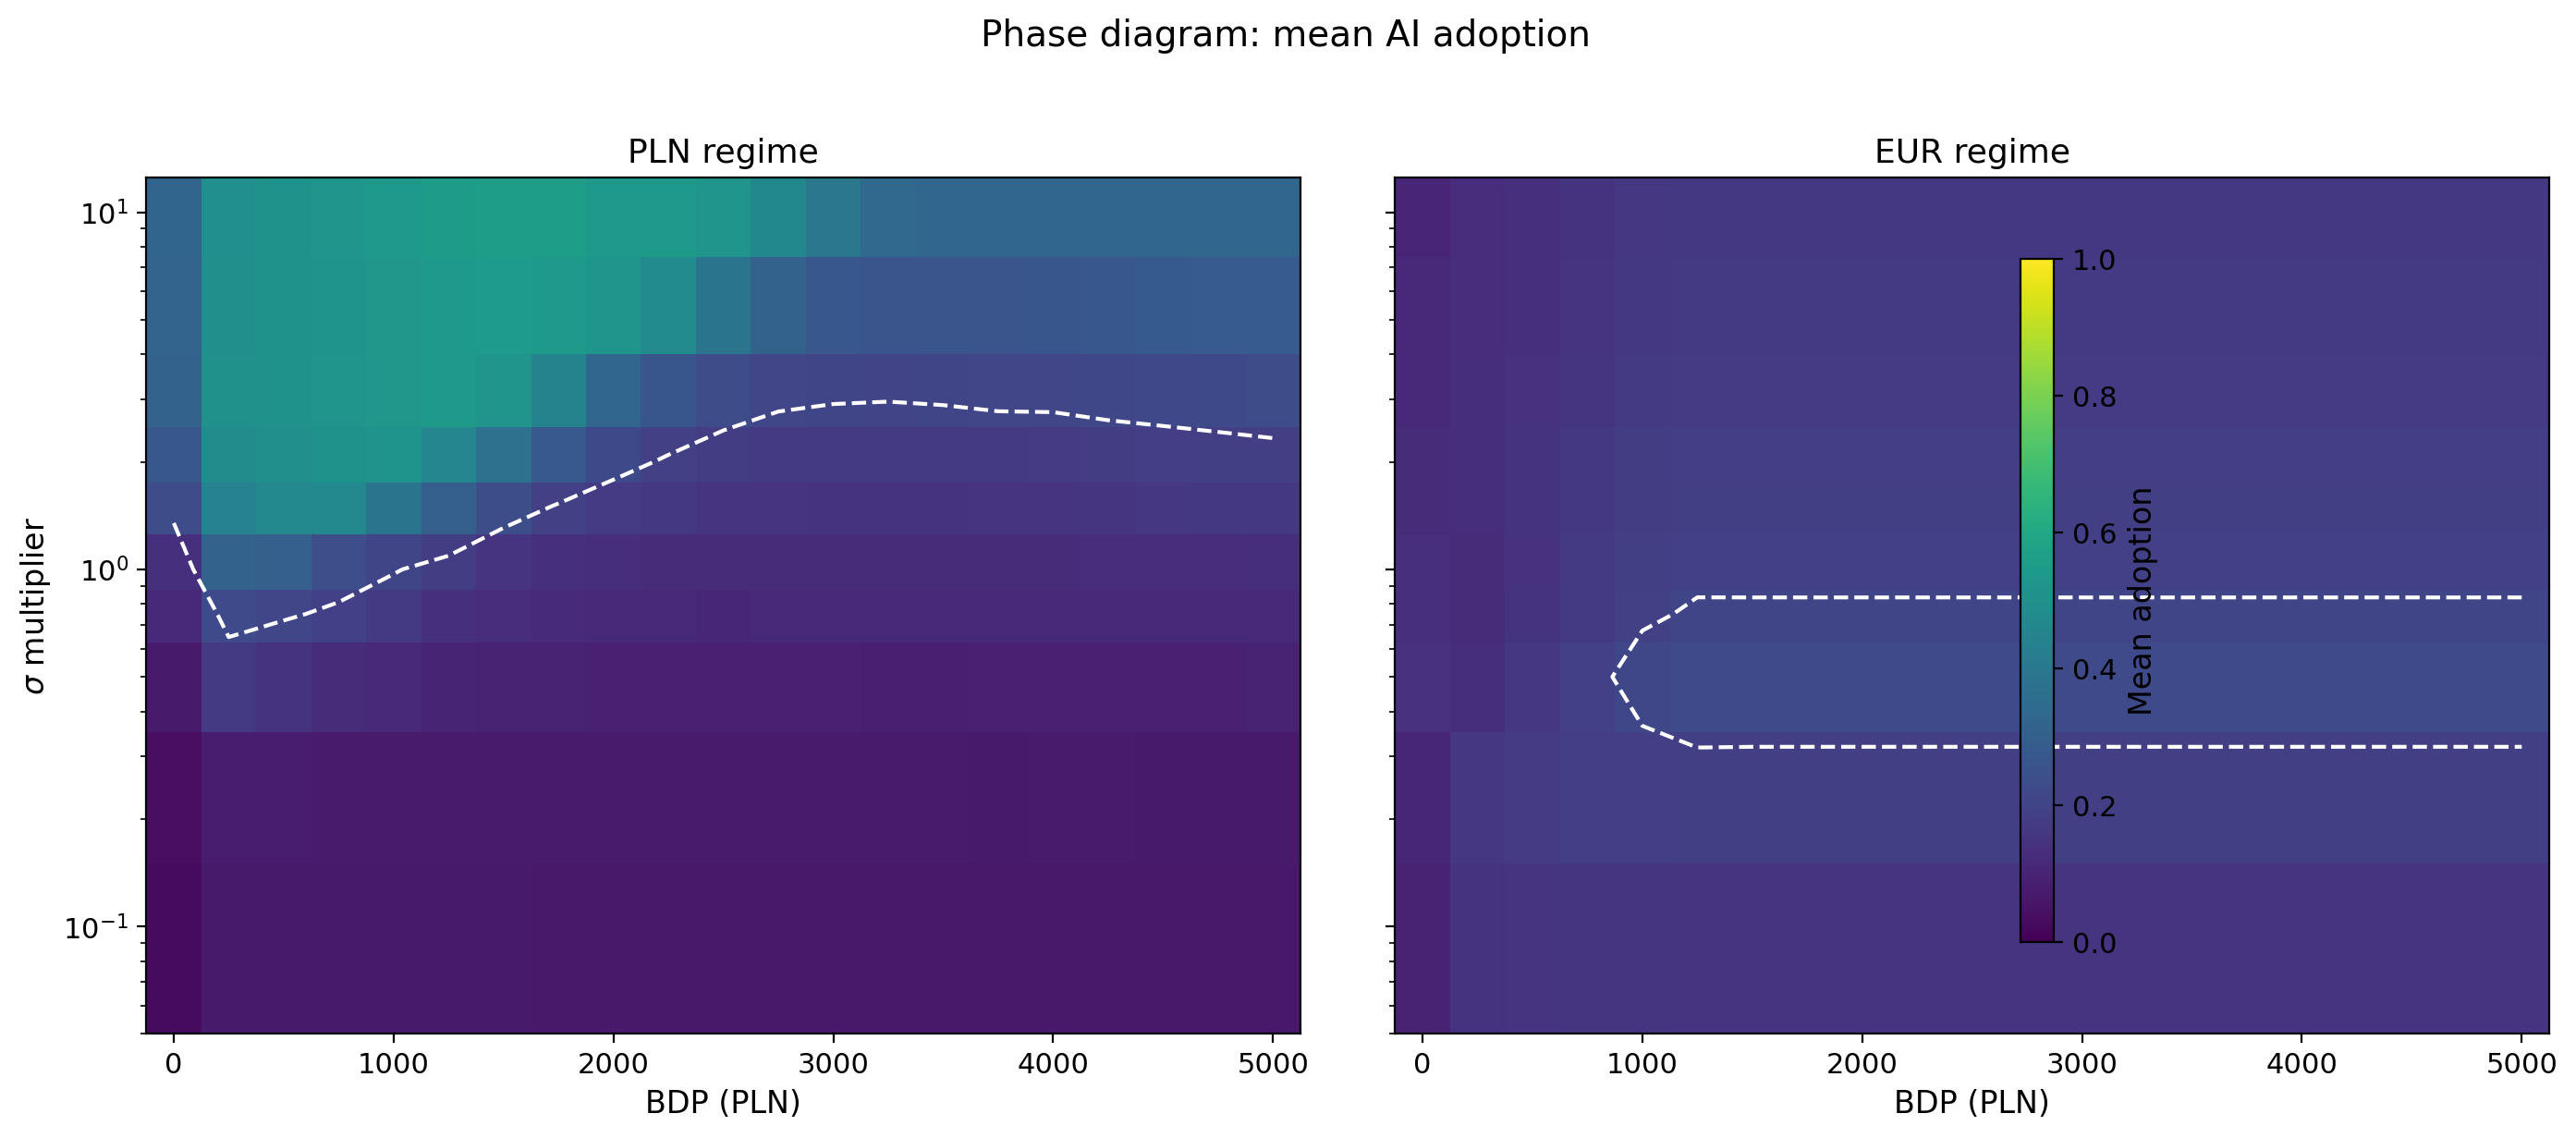
\includegraphics[width=0.85\textwidth]{../figures/fig01_phase_diagram.png}
    \caption{Phase diagram: mean adoption rate $\langle \phi \rangle$ in (BDP,
    $\sigma_{\mathrm{mult}}$) space for PLN (left) and EUR (right) regimes.
    The dashed white contour marks 20\% adoption. Under PLN, adoption peaks at
    low BDP and then \emph{declines}---a reentrant pattern. Under EUR, adoption
    forms a closed island bounded by SGP fiscal constraints.}
    \label{fig:heatmap}
\end{figure}

\textbf{PLN regime: reentrant adoption.} Under the floating PLN regime,
adoption does not increase monotonically with BDP. Instead, it exhibits a
pronounced \emph{reentrant} (inverted-U) profile: adoption rises from the
no-transfer baseline, peaks at $\mathrm{BDP} \approx 500$~PLN with
$\langle \phi \rangle \approx 0.30$ at $\sigma_{\mathrm{mult}} = 1.0$, and
then declines steadily toward $\langle \phi \rangle \approx 0.12$ at
$\mathrm{BDP} \geq 3{,}000$~PLN. The mechanism is as follows: at low BDP, the
transfer provides demand stimulus that improves firm profitability and
encourages automation investment; at high BDP, the fiscal expansion generates
inflation, triggering Taylor-rule interest rate hikes by the NBP, which raise
the cost of automation CAPEX financing and suppress adoption. The
\emph{maximum} of the adoption response thus defines an optimal fiscal
transfer---a finding with direct policy implications (Section~\ref{sec:policy}).

The reentrant shape is preserved across all $\sigma_{\mathrm{mult}}$ values,
though the peak height varies: at $\sigma_{\mathrm{mult}} = 5.0$, the peak
reaches $\langle \phi \rangle \approx 0.55$; at $\sigma_{\mathrm{mult}} =
0.2$, it barely exceeds 0.10.

\textbf{EUR regime: closed adoption island.} Under the EUR regime with SGP
constraints, the phase diagram takes a qualitatively different form. Adoption
is confined to a closed island in the region $\mathrm{BDP} \in [1{,}000,\;
3{,}000]$~PLN, $\sigma_{\mathrm{mult}} \in [0.3,\; 0.7]$. Outside this
island, either the fiscal space is insufficient (low BDP) or the SGP deficit
and debt limits choke the transfer before it can stimulate adoption
(high BDP). The island geometry is a direct consequence of the Maastricht
3\%/60\% thresholds documented in \textcite{Maciaszek2026b}.

\begin{figure}[htbp]
    \centering
    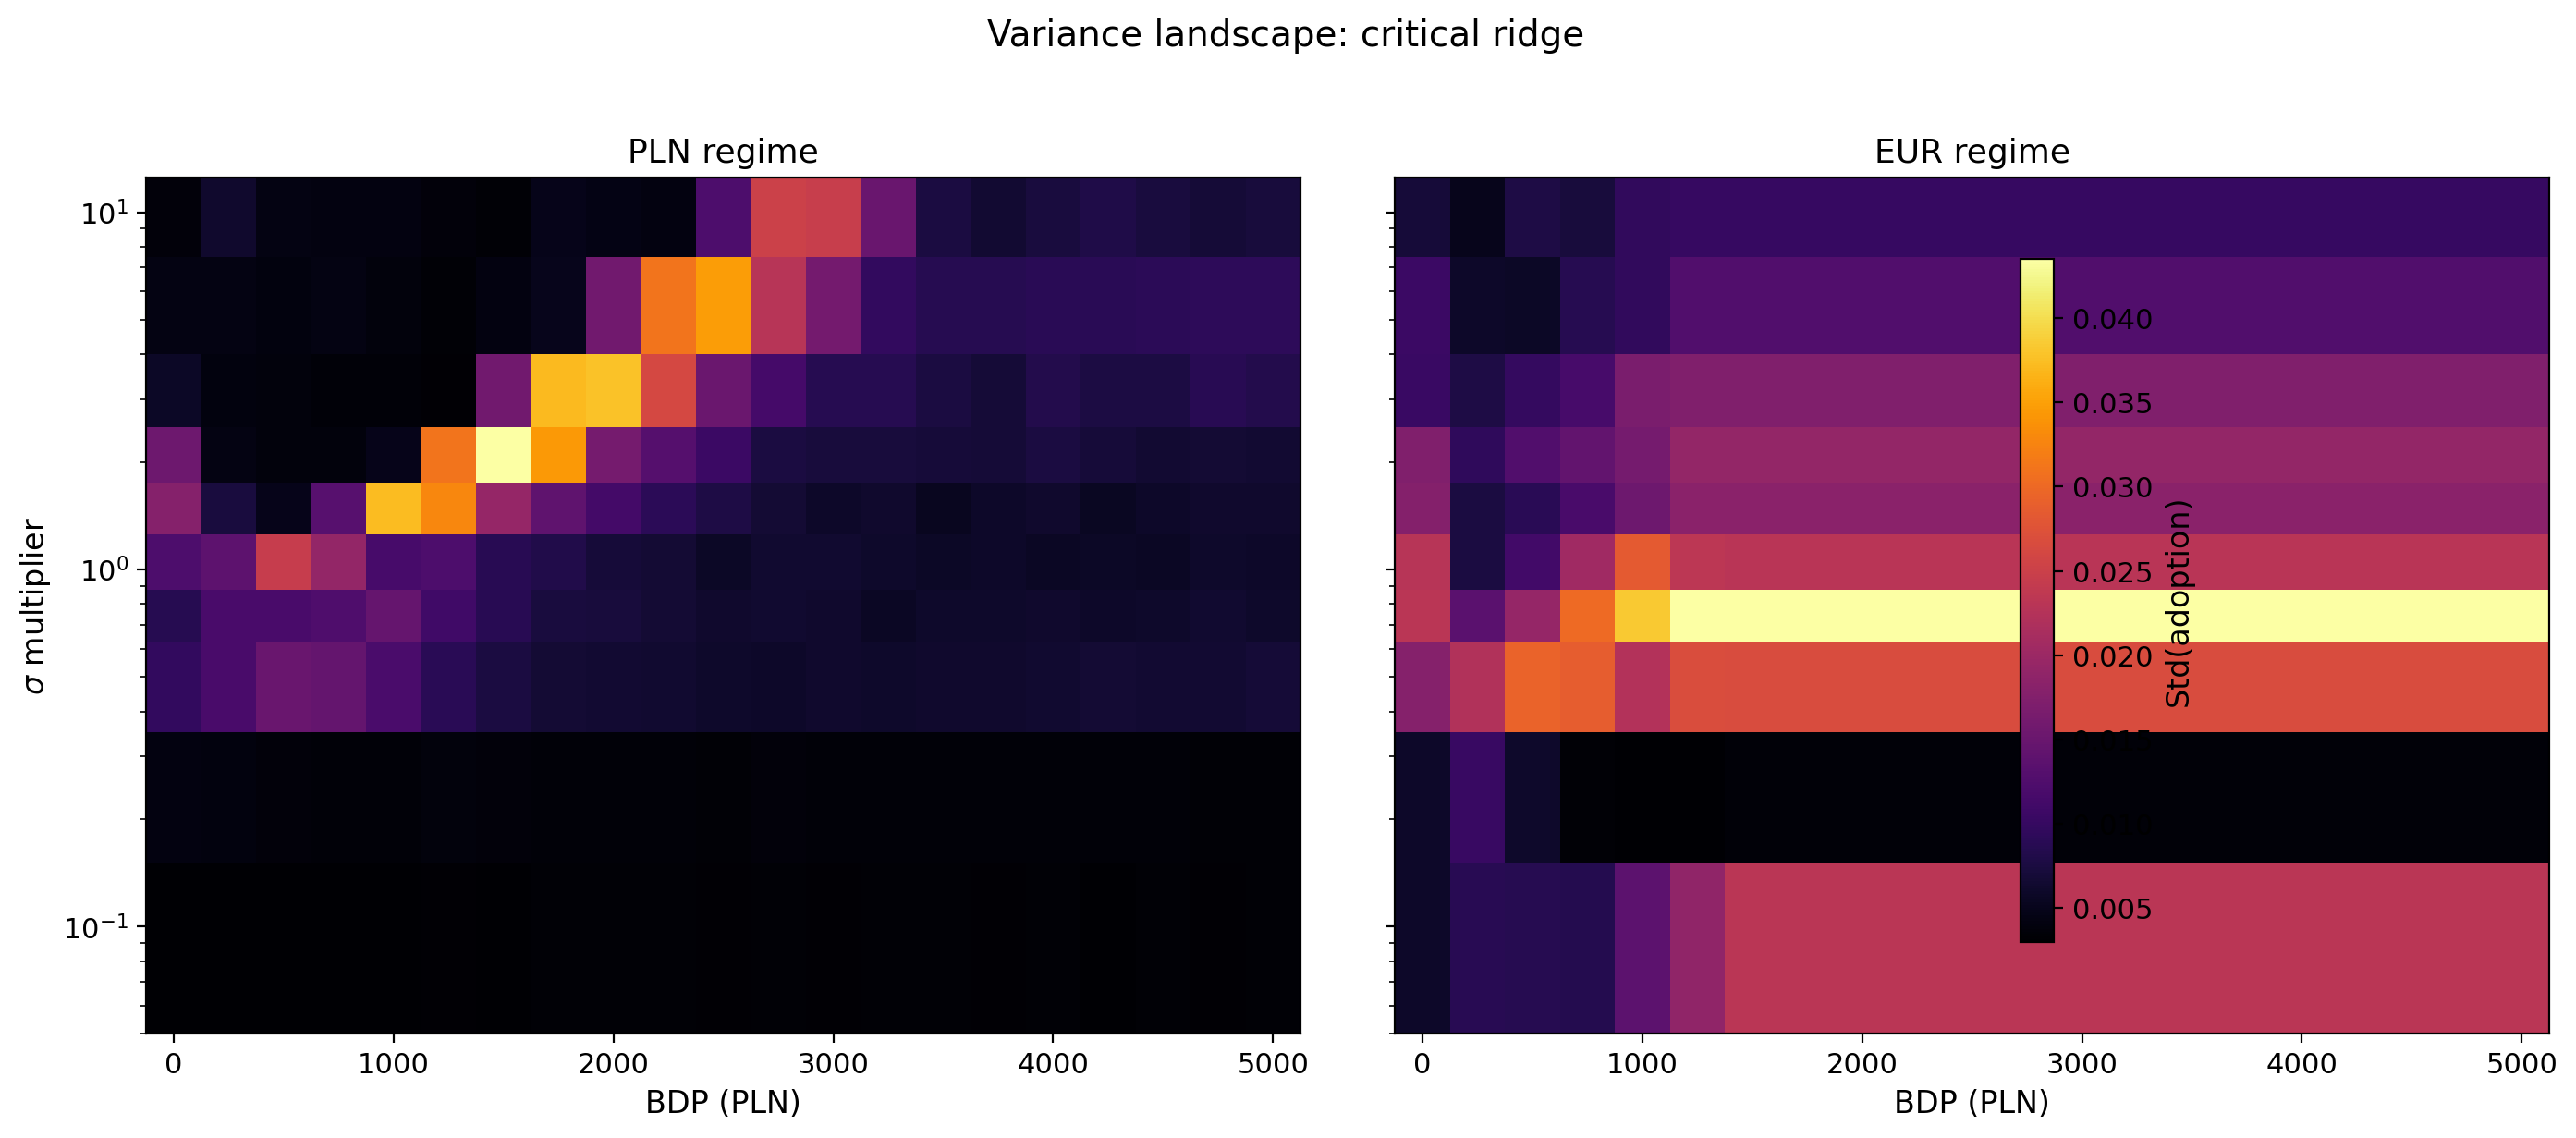
\includegraphics[width=0.85\textwidth]{../figures/fig02_variance_landscape.png}
    \caption{Cross-seed standard deviation of adoption rate in (BDP,
    $\sigma_{\mathrm{mult}}$) space. Under PLN (left), the variance ridge
    traces the reentrant peak at $\mathrm{BDP} \approx 500$~PLN. Under EUR
    (right), the variance concentrates in a narrow vertical stripe at
    $\mathrm{BDP} \approx 1{,}000$~PLN, consistent with the island boundary.}
    \label{fig:variance}
\end{figure}

Figure~\ref{fig:variance} shows the variance landscape. Under PLN, the
critical ``line'' is in fact a \emph{ridge} of maximum variance running along
$\mathrm{BDP} \approx 500$~PLN across all $\sigma_{\mathrm{mult}}$ values. The
ridge is broadest at intermediate $\sigma_{\mathrm{mult}}$ and narrows at
both extremes. Under EUR, the variance concentrates in a narrow vertical
stripe at $\mathrm{BDP} \approx 1{,}000$~PLN, marking the western boundary
of the adoption island where the SGP constraint begins to bind.

\begin{figure}[htbp]
    \centering
    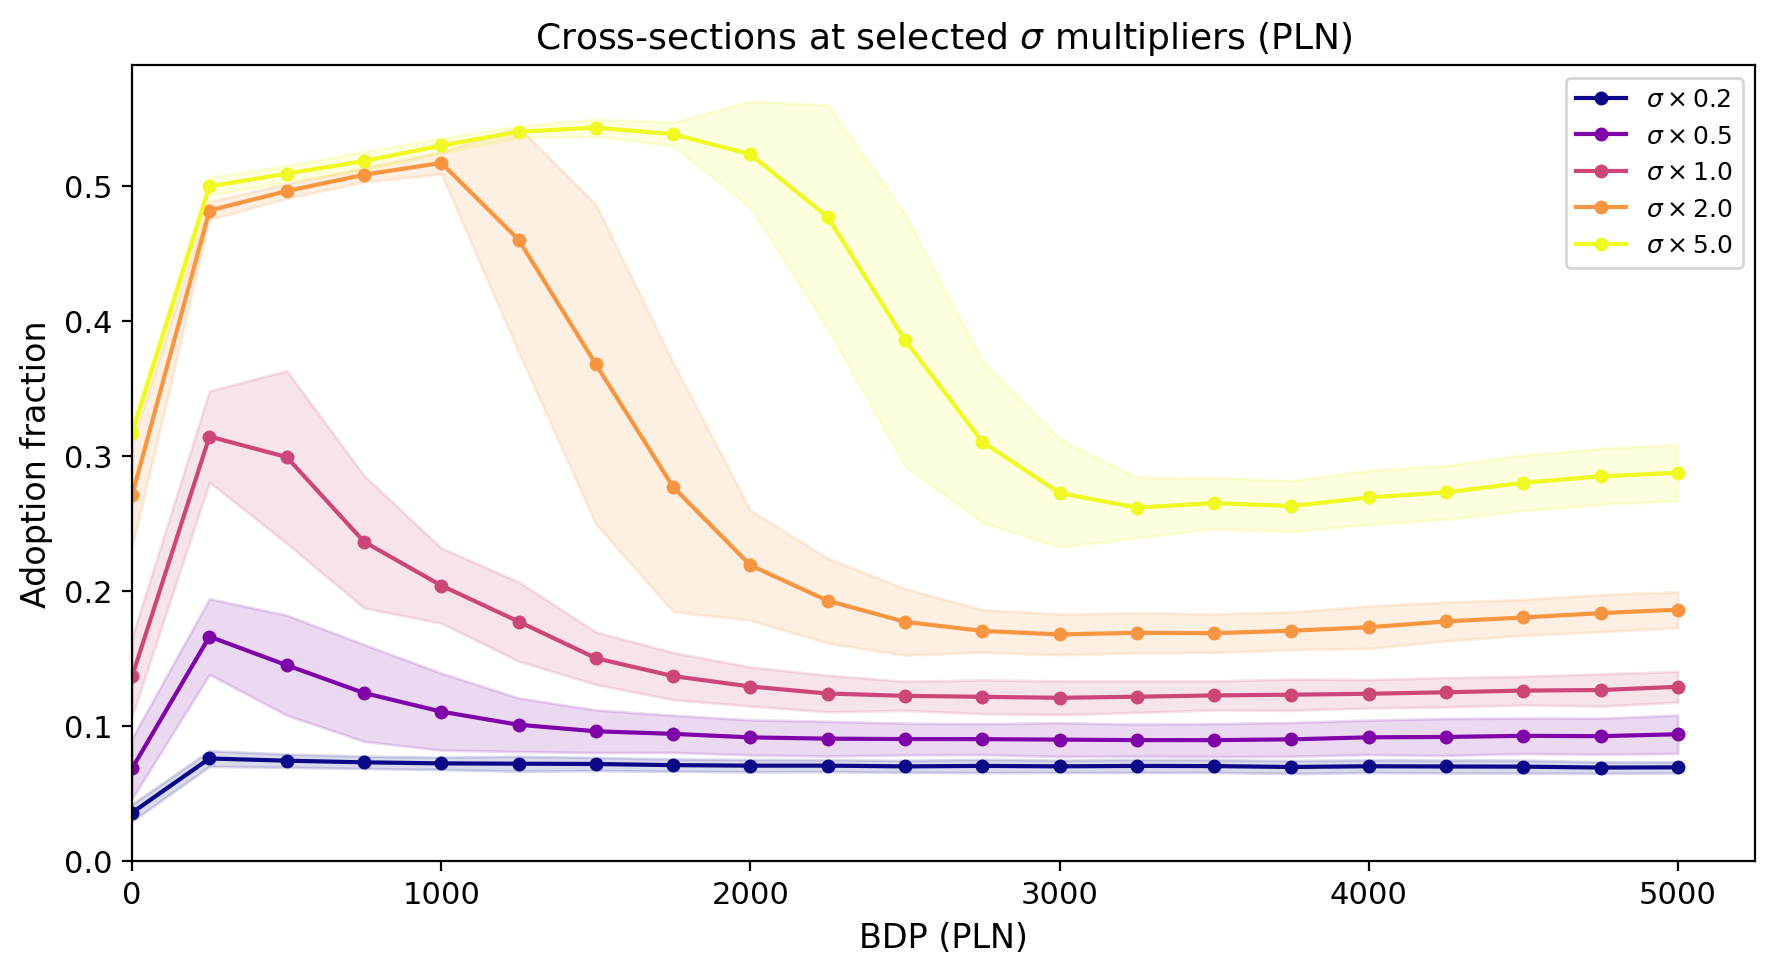
\includegraphics[width=0.85\textwidth]{../figures/fig03_cross_sections.png}
    \caption{Cross-sections of adoption rate vs.\ BDP at selected
    $\sigma_{\mathrm{mult}}$ values (PLN regime). All curves exhibit the
    reentrant inverted-U shape, with higher $\sigma_{\mathrm{mult}}$
    producing higher peak adoption but the same peak location
    ($\mathrm{BDP} \approx 500$~PLN).}
    \label{fig:cross_sections}
\end{figure}

Figure~\ref{fig:cross_sections} displays cross-sections at five
$\sigma_{\mathrm{mult}}$ slices ($\{0.2, 0.5, 1.0, 2.0, 5.0\}$). The key
observation is that all cross-sections share the same qualitative shape and
the same peak location ($\mathrm{BDP} \approx 500$~PLN), differing only in
amplitude. This confirms the Paper-03 finding that $\sigma$ modulates the
\emph{level} of adoption but not the \emph{critical threshold}: a 25-fold
change in $\sigma_{\mathrm{mult}}$ (from 0.2 to 5.0) shifts $\mathrm{BDP}_c$
by at most 250~PLN, compared to the 500--1{,}000~PLN shift induced by
switching from PLN to EUR \parencite{Maciaszek2026b}.

\subsection{Topology universality}
\label{sec:topology}

Figure~\ref{fig:topo_bifurcation} presents the bifurcation diagrams---mean
adoption rate $\langle \phi \rangle$ versus BDP---for the four network
topologies under both PLN and EUR regimes.

\begin{figure}[htbp]
    \centering
    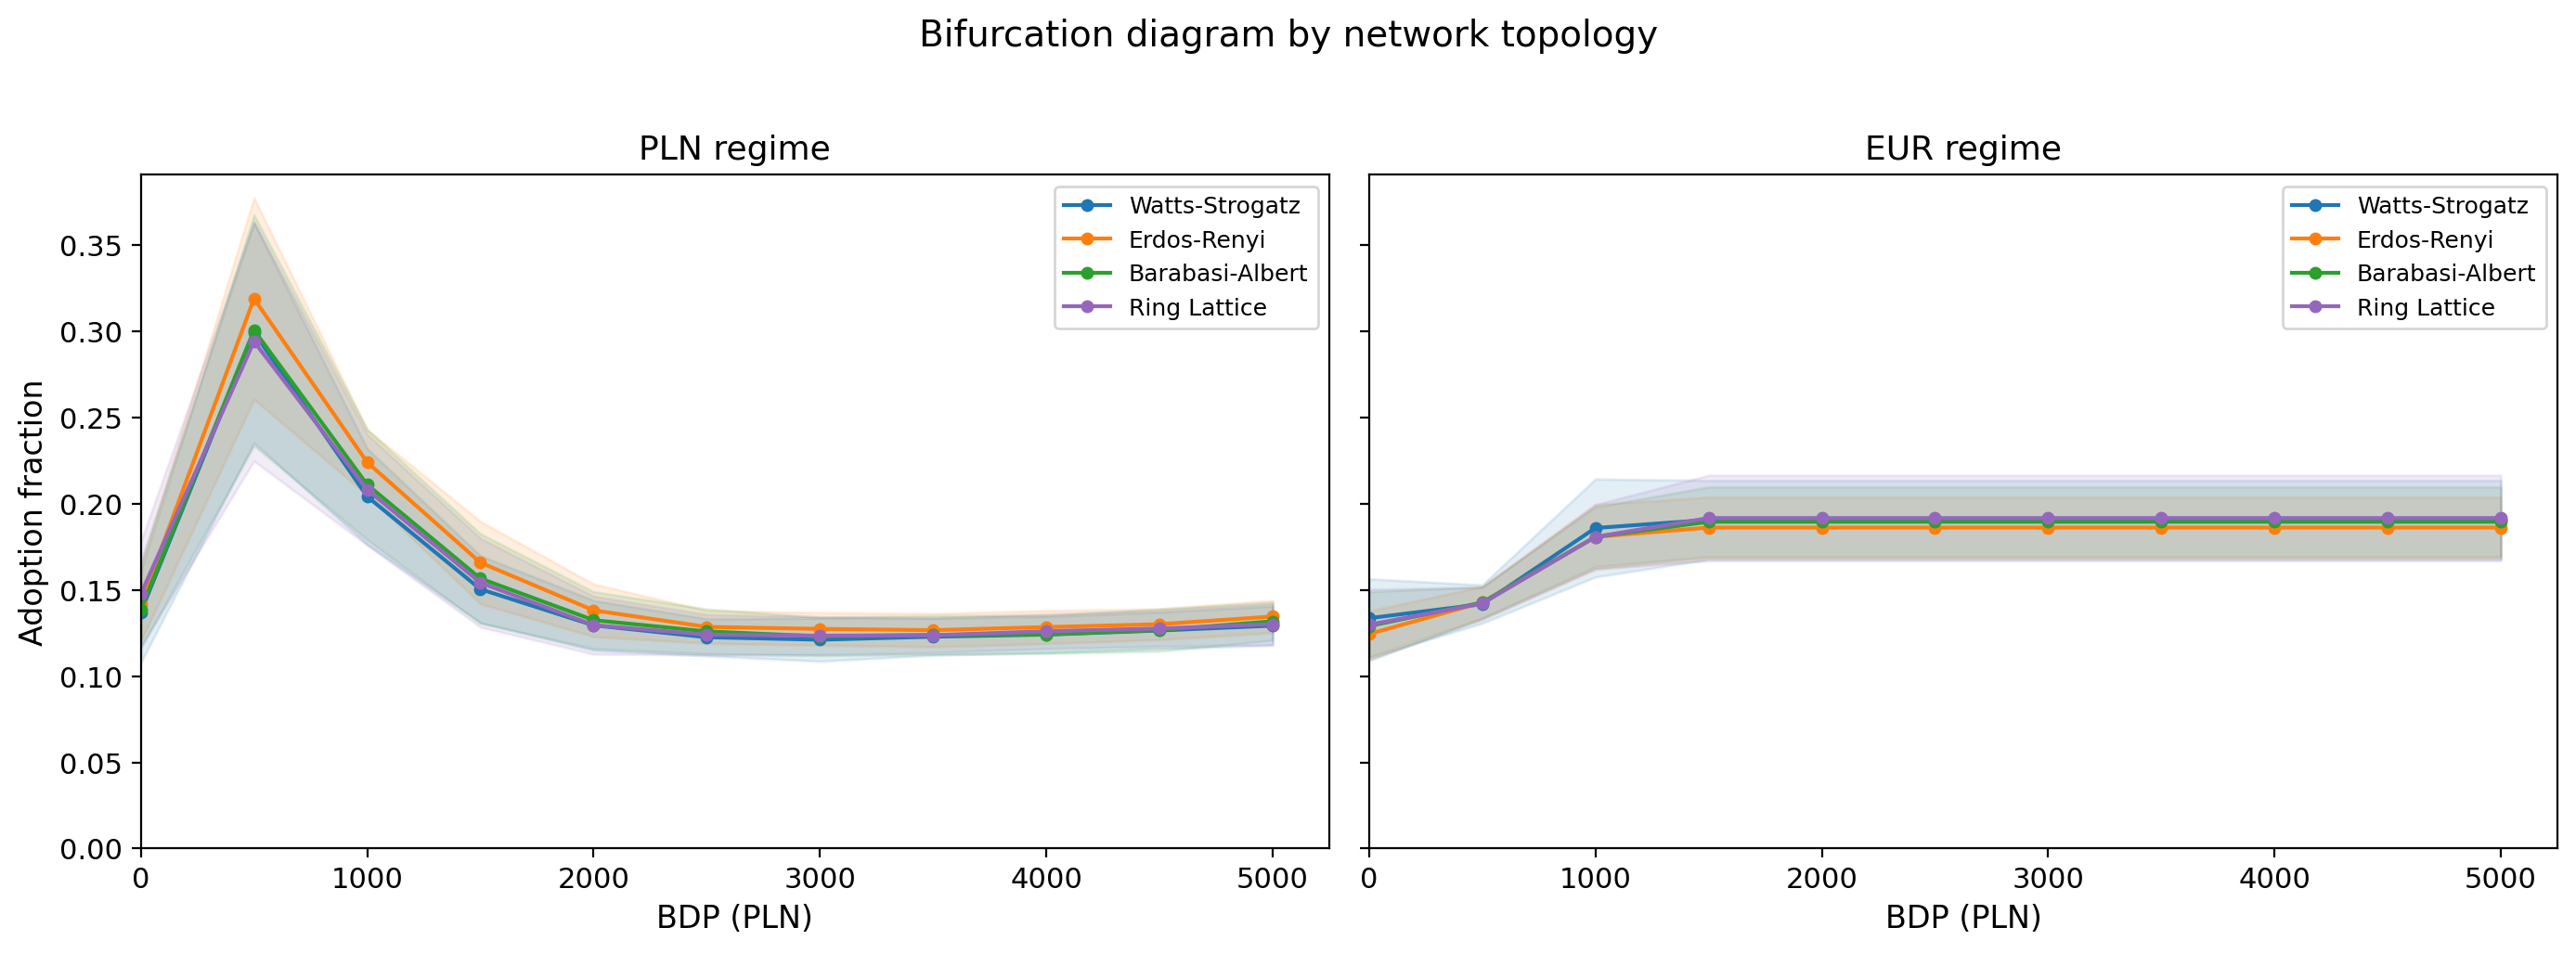
\includegraphics[width=0.85\textwidth]{../figures/fig04_topology_bifurcation.png}
    \caption{Bifurcation diagrams for Watts--Strogatz, Erd\H{o}s--R\'{e}nyi,
    Barab\'{a}si--Albert, and ring-lattice topologies under PLN (left) and EUR
    (right) regimes ($\sigma_{\mathrm{mult}} = 1.0$). Shaded bands show
    $\pm 1$ standard deviation across 30~seeds.}
    \label{fig:topo_bifurcation}
\end{figure}

The central finding is a striking \textbf{unanimity of the critical point under
PLN}: all four topologies yield $\mathrm{BDP}_c = 500$~PLN, with the
reentrant inverted-U curves overlapping almost perfectly. The peak adoption
rates are virtually indistinguishable ($\langle \phi \rangle \approx 0.30$),
and the variance envelopes are tightly aligned. This is perhaps the strongest
universality result in the paper: the critical point is determined entirely by
the macroeconomic feedback loop (BDP $\to$ demand $\to$ inflation $\to$ NBP
rate $\to$ investment cost $\to$ adoption), with the local network structure
playing no detectable role.

Under EUR, the critical points exhibit mild topology dependence:
$\mathrm{BDP}_c = 1{,}000$~PLN for WS and ER, and $\mathrm{BDP}_c =
1{,}500$~PLN for BA and ring lattice. The wider spread likely reflects the
interaction between the SGP fiscal constraint and the different variance
structures of each topology near the island boundary.

\begin{figure}[htbp]
    \centering
    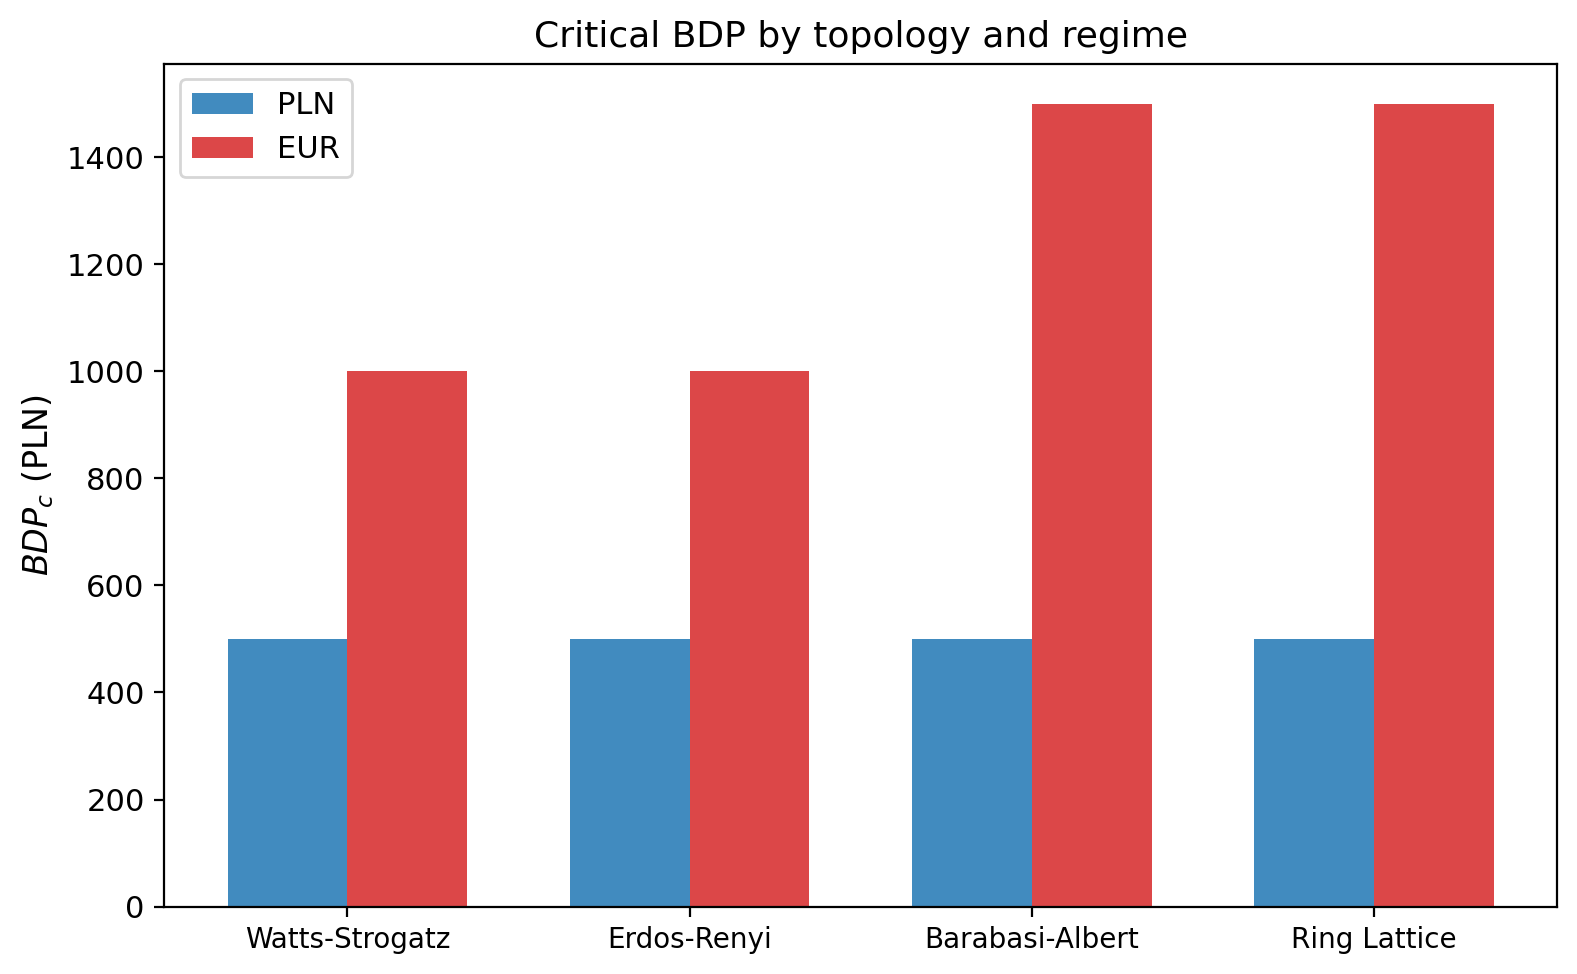
\includegraphics[width=0.85\textwidth]{../figures/fig05_critical_points.png}
    \caption{Critical BDP by topology and monetary regime, identified by the
    maximum-variance criterion. Under PLN, all four topologies agree on
    $\mathrm{BDP}_c = 500$~PLN. Under EUR, WS and ER yield
    $\mathrm{BDP}_c = 1{,}000$~PLN while BA and ring lattice yield
    $\mathrm{BDP}_c = 1{,}500$~PLN.}
    \label{fig:critical_points}
\end{figure}

Figure~\ref{fig:critical_points} summarizes the critical-point comparison.
The perfect PLN unanimity across four qualitatively different network
topologies---ranging from the highly clustered ring lattice (purely local
interactions) to the hub-dominated BA graph (extreme heterogeneity)---is a
strong indicator of universality. In the renormalization group framework,
this means that the local interaction topology is an \emph{irrelevant variable}:
it does not affect the critical behavior because the global fiscal feedback
dominates the dynamics.

\subsection{Critical exponents}
\label{sec:exponents}

We extract the susceptibility exponent $\gamma/2$ from log--log fits of
$\mathrm{std}[\phi]$ versus $|\mathrm{BDP} - \mathrm{BDP}_c|$ near the
identified critical points. Figure~\ref{fig:loglog} shows the log--log scatter
with reference slopes for the mean-field ($\gamma/2 = 0.5$), 2D~Ising
($\gamma/2 = 0.875$), and percolation ($\gamma/2 \approx 1.2$) universality
classes.

\begin{figure}[htbp]
    \centering
    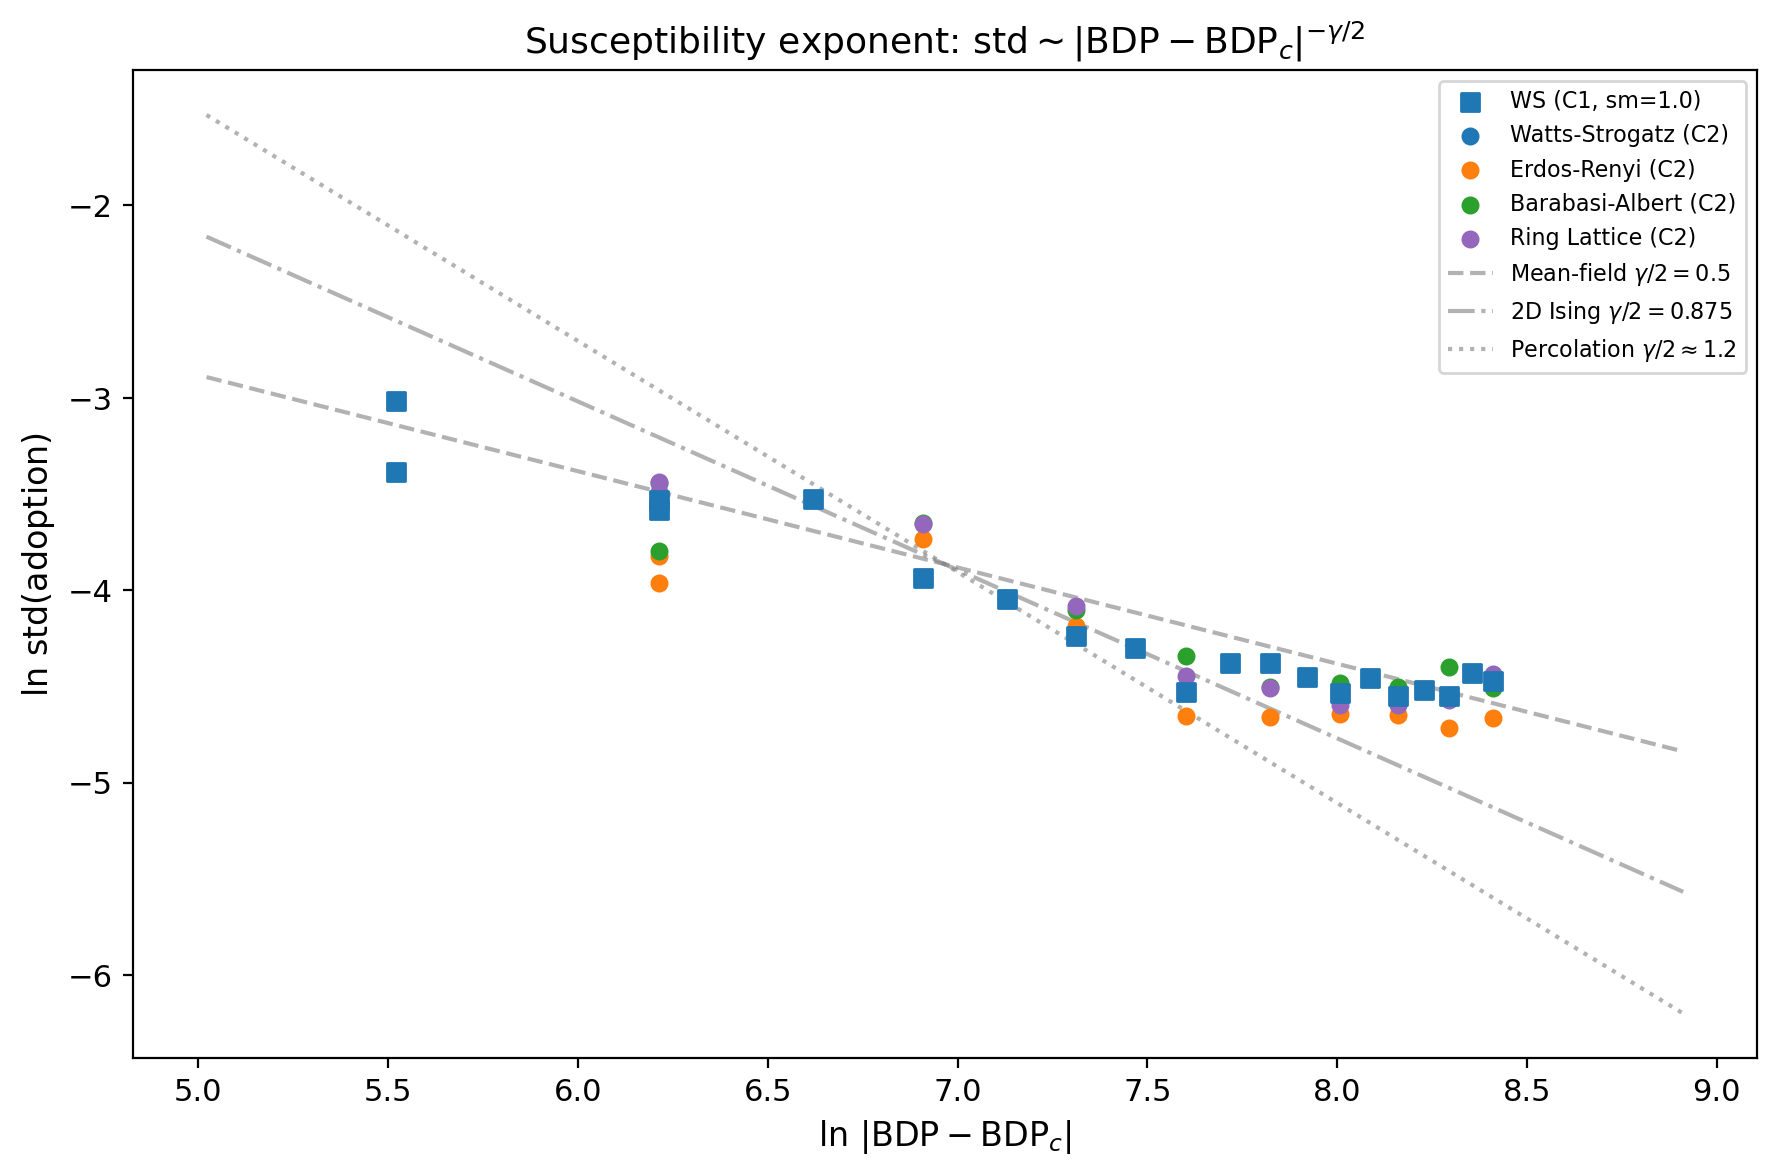
\includegraphics[width=0.85\textwidth]{../figures/fig06_critical_exponents.png}
    \caption{Log--log scaling of cross-seed adoption standard deviation vs.\
    $|\mathrm{BDP} - \mathrm{BDP}_c|$ for five topology/campaign combinations
    (PLN regime). Reference lines show the expected slopes for mean-field,
    2D~Ising, and percolation universality classes.}
    \label{fig:loglog}
\end{figure}

Table~\ref{tab:exponents} reports the estimated $\gamma/2$ values and their
$R^2$ statistics.

\begin{table}[htbp]
\centering
\caption{Estimated susceptibility exponent $\gamma/2$ from log--log fits.
The mean-field reference value is $\gamma/2 = 0.5$; 2D~Ising gives 0.875
and percolation $\approx 1.2$. WS and lattice estimates bracket the
mean-field value with high $R^2$.}
\label{tab:exponents}
\begin{tabular}{lccc}
\toprule
Dataset & $\hat{\gamma}/2$ & $R^2$ & Implied $\hat{\gamma}$ \\
\midrule
WS (C1, $\sigma_{\mathrm{mult}} = 1.0$) & 0.539 & 0.87 & 1.08 \\
WS (C2) & 0.606 & 0.99 & 1.21 \\
Ring lattice (C2) & 0.510 & 0.89 & 1.02 \\
Barab\'{a}si--Albert (C2) & 0.364 & 0.50 & 0.73 \\
Erd\H{o}s--R\'{e}nyi (C2) & 0.173 & 0.23 & 0.35 \\
\midrule
Mean-field reference & 0.500 & --- & 1.00 \\
\bottomrule
\end{tabular}
\end{table}

\begin{figure}[htbp]
    \centering
    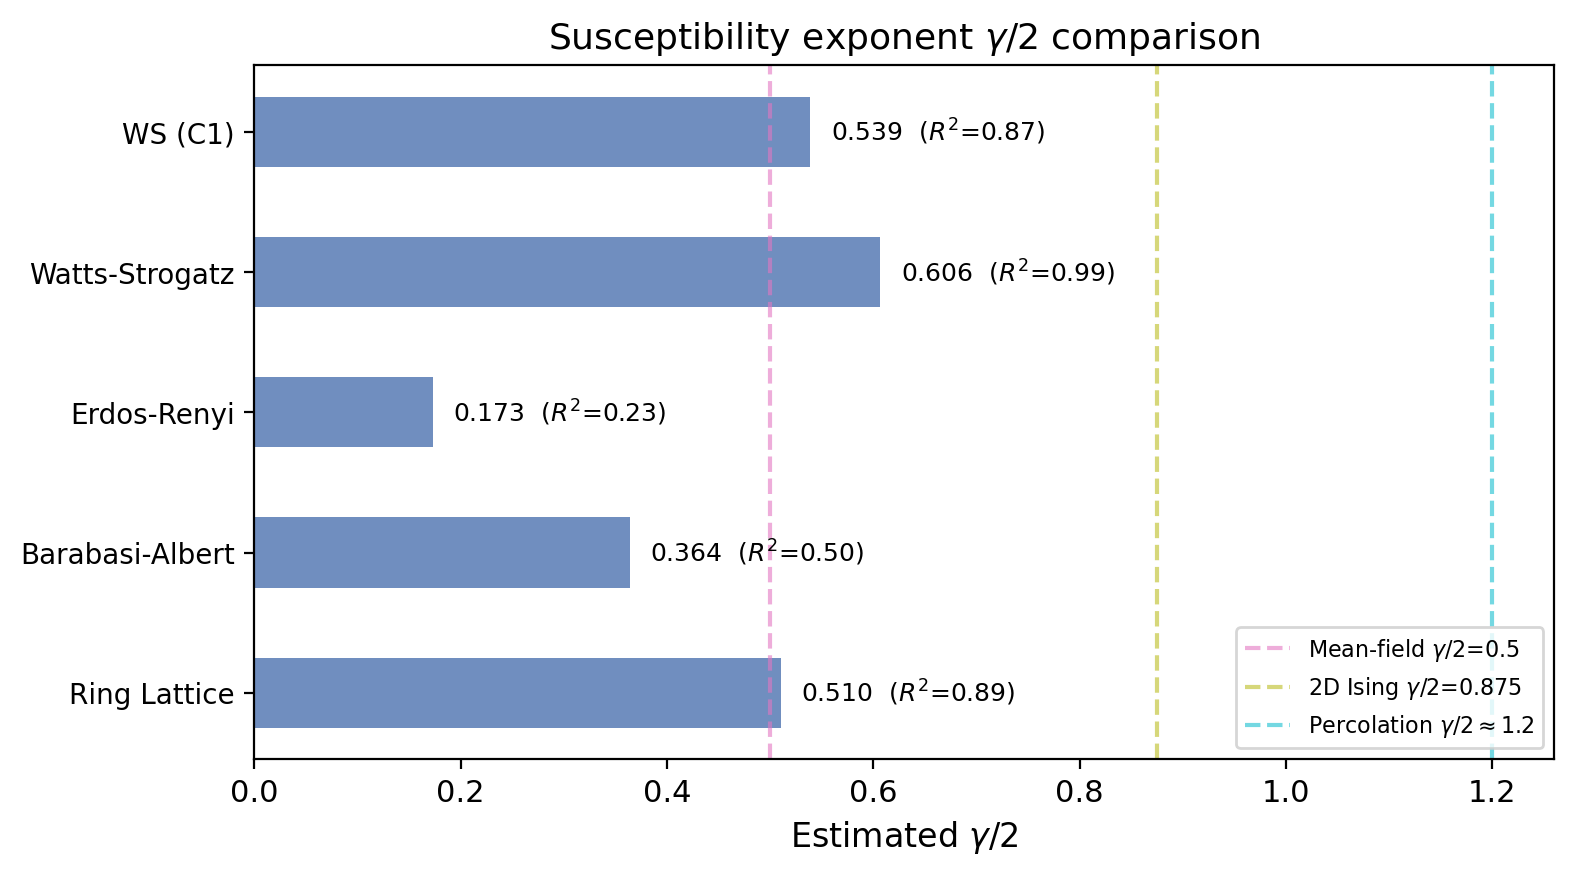
\includegraphics[width=0.85\textwidth]{../figures/fig07_exponent_forest.png}
    \caption{Forest plot of estimated $\gamma/2$ values with $R^2$ annotations.
    The vertical dashed lines mark reference values for the mean-field,
    2D~Ising, and percolation universality classes.}
    \label{fig:forest}
\end{figure}

Figure~\ref{fig:forest} displays the exponent estimates as a forest plot. The
three best-resolved datasets---WS~(C1), WS~(C2), and ring lattice---yield
$\gamma/2 \in [0.51, 0.61]$ with $R^2 \geq 0.87$, implying $\gamma \approx
1.0$--$1.2$. These values bracket the mean-field reference $\gamma = 1.0$,
supporting a \textbf{mean-field universality class} assignment. The BA and ER
estimates are less reliable ($R^2 \leq 0.50$), likely because the coarser
BDP grid in Campaign~2 (step 500~PLN vs.\ 250~PLN in Campaign~1) provides
fewer points in the scaling region near $\mathrm{BDP}_c$.

\subsection{Finite-size scaling}
\label{sec:fss}

Campaign~3 provides the data for FSS analysis.
Figure~\ref{fig:susceptibility} shows the susceptibility $\chi = N \,
\mathrm{Var}[\phi]$ as a function of BDP for the five system sizes.

\begin{figure}[htbp]
    \centering
    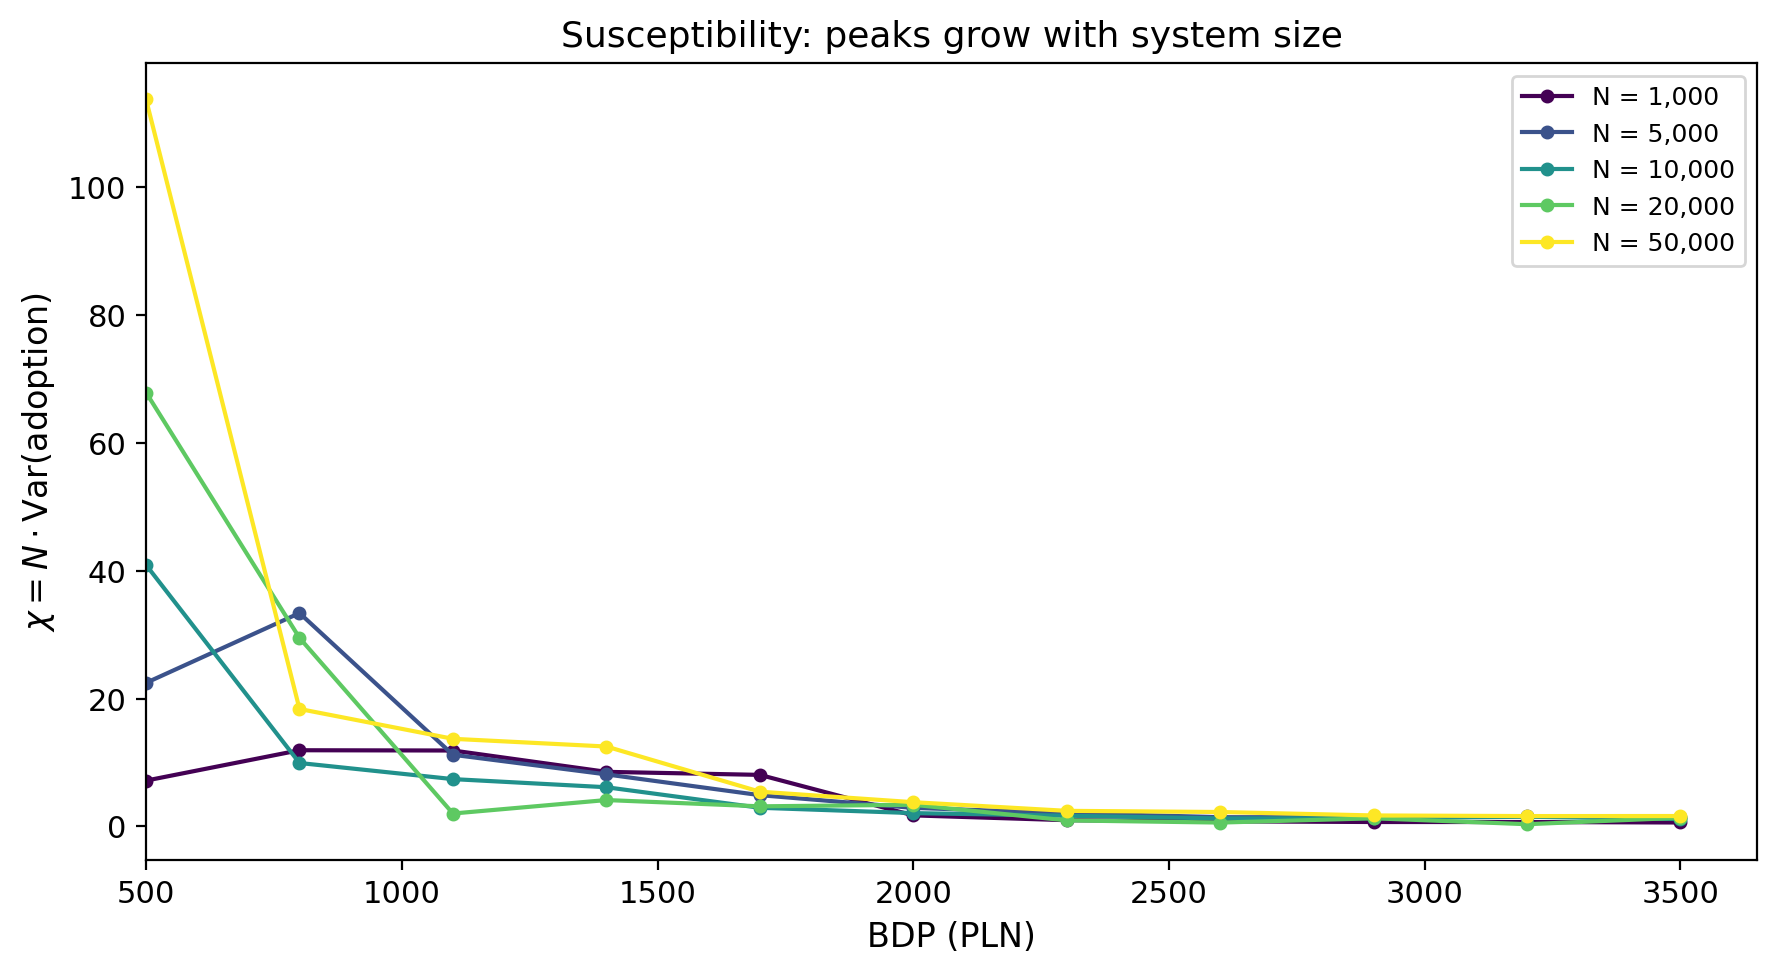
\includegraphics[width=0.85\textwidth]{../figures/fig08_susceptibility.png}
    \caption{Susceptibility $\chi = N \, \mathrm{Var}[\phi]$ vs.\ BDP for
    $N \in \{1{,}000,\; 5{,}000,\; 10{,}000,\; 20{,}000,\; 50{,}000\}$. The
    peak height grows systematically with system size ($\chi_{\max} \approx 12,
    33, 40, 68, 112$ for increasing~$N$), confirming a genuine collective
    effect.}
    \label{fig:susceptibility}
\end{figure}

The susceptibility peak grows monotonically with $N$: $\chi_{\max} \approx 12$
(N = 1{,}000), 33 (5{,}000), 40 (10{,}000), 68 (20{,}000), and 112
(50{,}000). This systematic growth confirms that the variance peak is not a
finite-size artifact---it sharpens and amplifies as the system grows,
consistent with a divergent susceptibility in the thermodynamic limit.

\textbf{Critical-point convergence.} Figure~\ref{fig:bdpc_conv} shows
$\mathrm{BDP}_c(N)$ as a function of system size. Rather than the smooth
power-law convergence $\mathrm{BDP}_c(N) - \mathrm{BDP}_c(\infty) \sim
N^{-1/\bar{\nu}}$ predicted by the standard FSS ansatz, we observe a
\emph{discrete jump}: $\mathrm{BDP}_c = 800$~PLN for $N \leq 5{,}000$,
dropping abruptly to $\mathrm{BDP}_c = 500$~PLN for $N \geq 10{,}000$, where
it remains stable through $N = 50{,}000$. This step-function behavior suggests
a \textbf{crossover} between two competing regimes---a finite-size regime
where network-level fluctuations dominate, and a thermodynamic regime where
the macroeconomic feedback loop pins the critical point.

\begin{figure}[htbp]
    \centering
    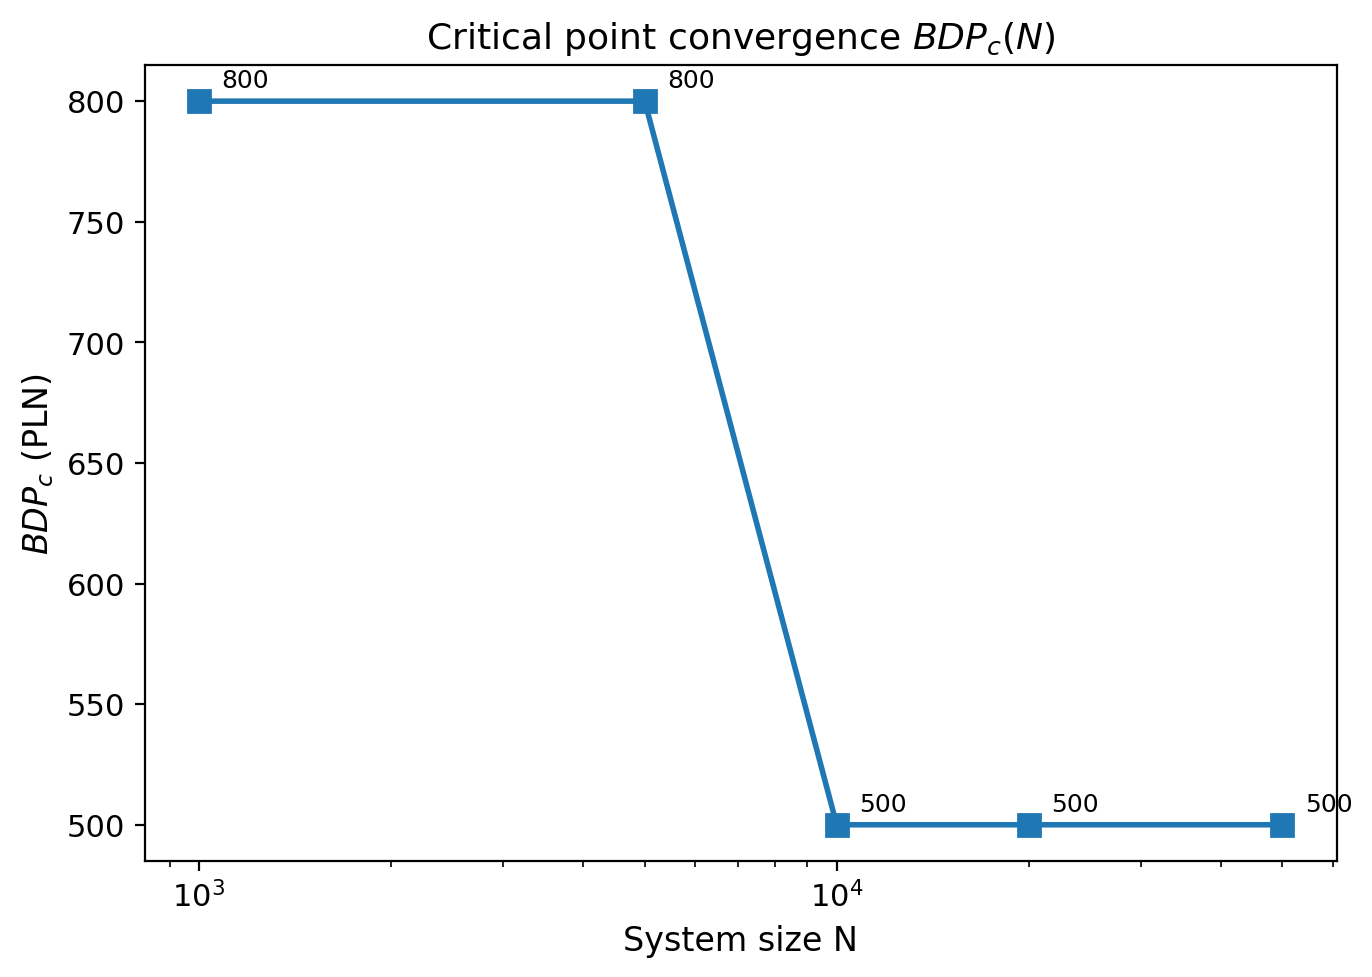
\includegraphics[width=0.70\textwidth]{../figures/fig10_bdpc_convergence.png}
    \caption{Critical-point convergence $\mathrm{BDP}_c(N)$. The critical BDP
    jumps discretely from 800~PLN ($N \leq 5{,}000$) to 500~PLN
    ($N \geq 10{,}000$) rather than converging smoothly, indicating a crossover
    between finite-size and thermodynamic regimes.}
    \label{fig:bdpc_conv}
\end{figure}

\textbf{Data collapse.} Figure~\ref{fig:collapse} shows the best-fit data
collapse obtained by optimizing the rescaling exponents $1/\bar{\nu}$ and
$\gamma/\bar{\nu}$ in equation~\eqref{eq:collapse} via differential evolution.
The optimizer converges to $1/\bar{\nu} = 0.77$ and $\gamma/\bar{\nu} = 3.0$,
but the latter hits the upper bound of the search range, indicating that the
collapse is \emph{partial}. Visually, the $N = 5{,}000$ through $N = 50{,}000$
curves overlap reasonably well, but the $N = 1{,}000$ curve separates
distinctly from the rest.

\begin{figure}[htbp]
    \centering
    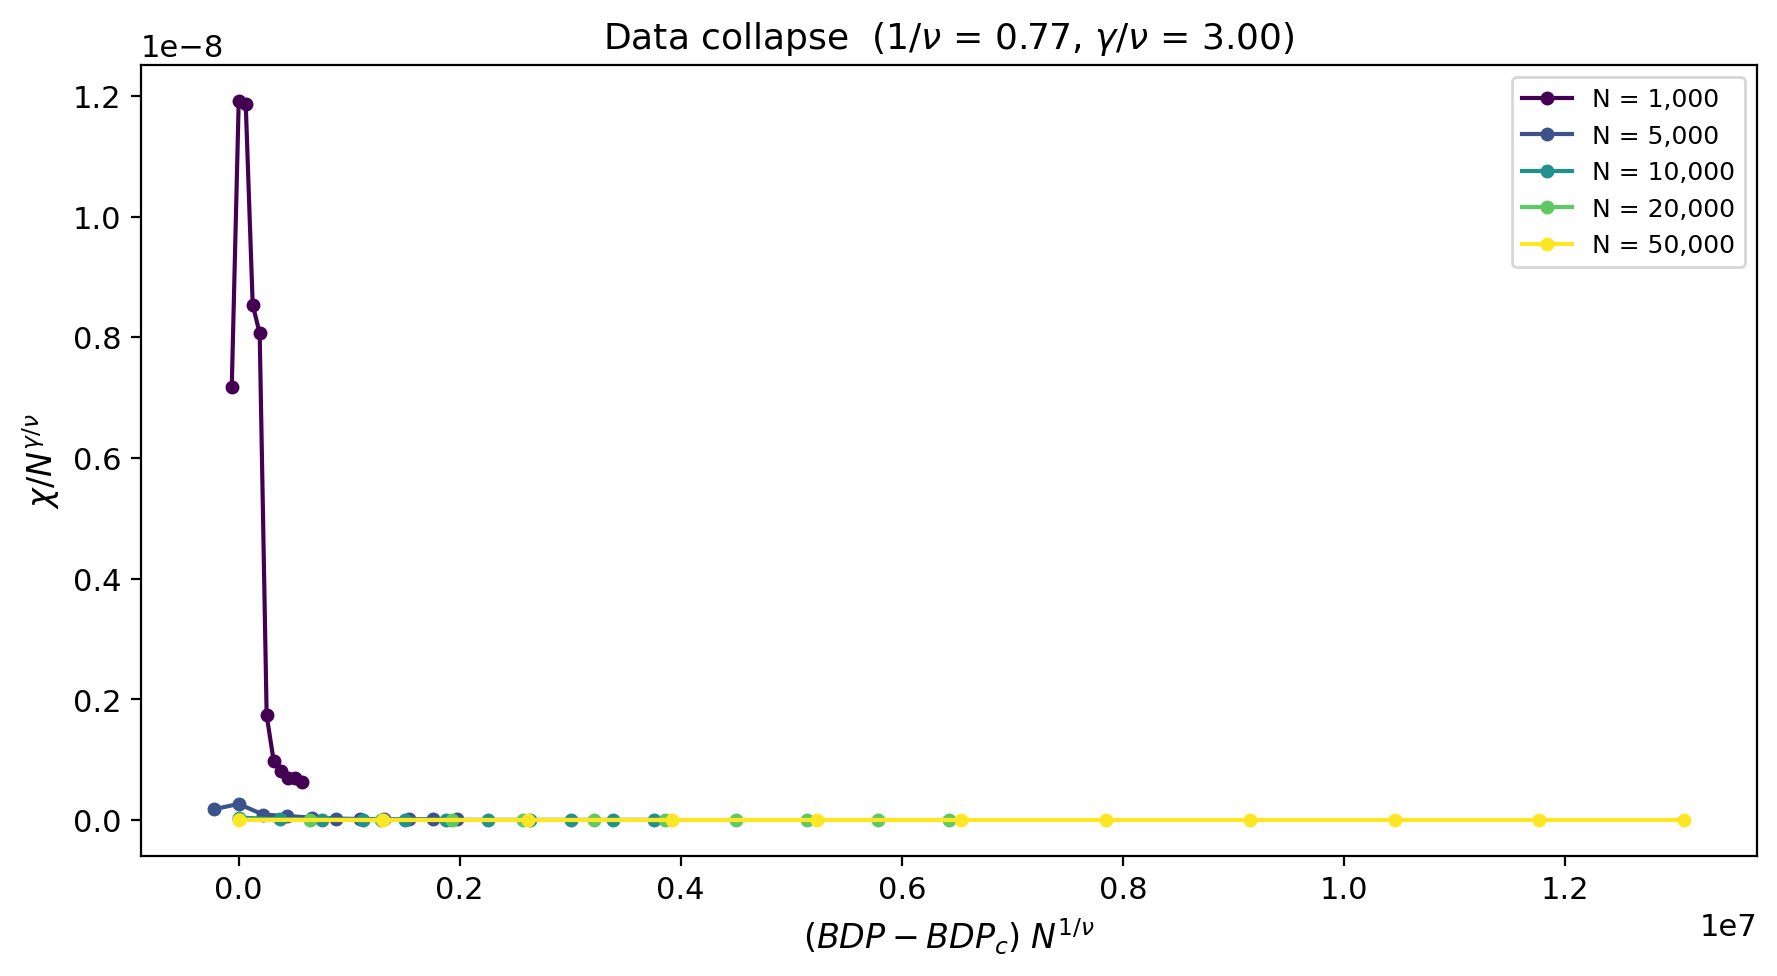
\includegraphics[width=0.85\textwidth]{../figures/fig09_data_collapse.png}
    \caption{Finite-size scaling data collapse. Susceptibility curves are
    rescaled according to equation~\eqref{eq:collapse} with optimized
    exponents $1/\bar{\nu} = 0.77$, $\gamma/\bar{\nu} = 3.0$. The collapse
    is partial: $N \geq 5{,}000$ curves overlap, but $N = 1{,}000$ separates
    distinctly.}
    \label{fig:collapse}
\end{figure}

The partial collapse is consistent with the discrete $\mathrm{BDP}_c(N)$
jump: the standard FSS ansatz assumes a smooth, scale-free approach to the
thermodynamic limit, which is violated when the system crosses over between
qualitatively different regimes. We interpret this as evidence that the model
produces a genuine collective effect (growing $\chi_{\max}$) but does not
conform to the simple second-order phase transition template. The implications
for the universality classification are discussed in
Section~\ref{sec:discussion}.

\subsection{Decision rule robustness}
\label{sec:decision}

Campaign~4 tests whether the reentrant profile and critical point are artifacts
of the specific functional form of the firm adoption decision rule.

\begin{figure}[htbp]
    \centering
    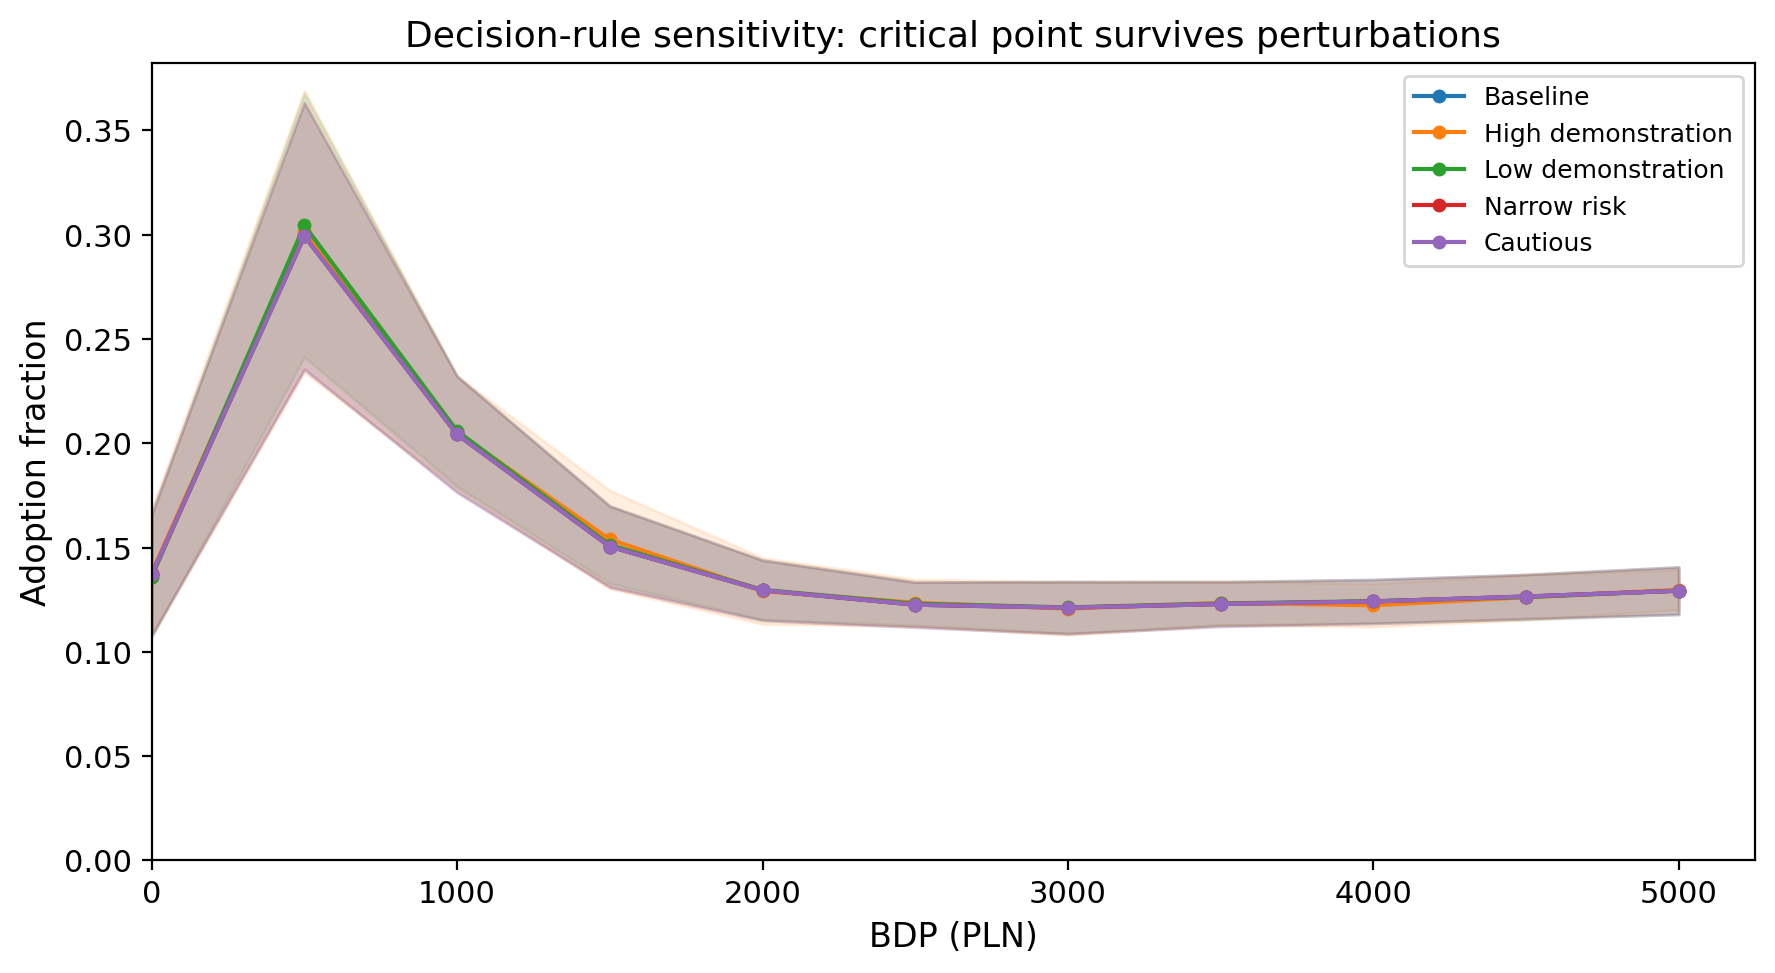
\includegraphics[width=0.85\textwidth]{../figures/fig11_decision_sensitivity.png}
    \caption{Bifurcation diagrams under five decision-rule variants: baseline,
    high demographic weighting, low demographic weighting, narrow risk-aversion
    band, and cautious (elevated) adoption threshold. All five variants produce
    nearly identical curves with $\mathrm{BDP}_c = 500$~PLN and peak adoption
    $\approx 30\%$.}
    \label{fig:decision}
\end{figure}

Figure~\ref{fig:decision} shows the bifurcation diagrams for the five
decision-rule variants. The result is unequivocal: all five curves are
\emph{nearly identical}. Not only does the critical point remain at
$\mathrm{BDP}_c = 500$~PLN across all variants, but the entire reentrant
profile---peak height ($\approx 30\%$), decline rate, and variance
envelope---is preserved. This goes substantially beyond the typical robustness
finding of ``the critical point shifts but survives''; here, the critical point
and the full bifurcation curve are \emph{completely invariant} to the
decision-rule perturbations tested.

This invariance confirms that the reentrant adoption pattern is an emergent
consequence of the macroeconomic feedback loop
(BDP $\to$ demand $\to$ inflation $\to$ interest rate $\to$ CAPEX cost $\to$
adoption), not a fine-tuned artifact of a particular parameterization of the
firm-level decision rule.

%======================================================================
\section{Discussion}
\label{sec:discussion}
%======================================================================

\subsection{Universality class interpretation}
\label{sec:universality}

The estimated susceptibility exponents $\gamma/2 \in [0.51, 0.61]$ for the
well-resolved datasets (WS and ring lattice) imply $\gamma \approx 1.0$--$1.2$,
placing the model in or near the \textbf{mean-field universality class}
($\gamma_{\mathrm{MF}} = 1.0$). This classification has a natural
interpretation: the global fiscal feedback effectively makes all firms interact
with all others through the macroeconomic channel. Each firm's profitability
depends on aggregate demand, which depends on the BDP transfer and its
inflationary consequences---both of which are economy-wide variables,
independent of local network position. This global coupling washes out the
local network structure, explaining both the mean-field exponents and the
perfect topology universality of $\mathrm{BDP}_c$.

The topology independence documented in Section~\ref{sec:topology} is
directly consistent with this interpretation. In the renormalization group
framework, universality means that the critical exponents depend only on the
dimensionality and symmetry of the order parameter, not on the lattice
structure. Our finding that WS, ER, BA, and ring-lattice topologies yield the
same $\mathrm{BDP}_c$ and compatible exponents is precisely the empirical
signature of universality \parencite{Stanley1971,Fisher1998}.

The effective dimension of the model is governed by the macroeconomic feedback,
which is global (infinite-range). For systems above the upper critical
dimension ($d_c = 4$ for Ising-like models), mean-field exponents hold
regardless of the local network structure
\parencite{Castellano2009,Binder2010}. Since the WS and ER networks already
have effective dimension $d \to \infty$ (mean path length $\sim \log N$), and
the BA and lattice networks are coupled to the same global fiscal channel, all
topologies are effectively above~$d_c$, consistent with mean-field behavior.

\subsection{Policy implications: the optimal BDP}
\label{sec:policy}

The reentrant adoption profile has a sharp policy implication: there exists an
\textbf{optimal BDP} that maximizes technology adoption, and increasing the
transfer beyond this optimum is \emph{counterproductive}. Under the PLN regime,
this optimum lies at approximately 500~PLN/month.

The mechanism is transparent. At $\mathrm{BDP} = 500$~PLN, the demand stimulus
is large enough to improve firm profitability and encourage automation
investment, but small enough that the resulting inflationary pressure remains
manageable under the Taylor rule. Beyond 500~PLN, the fiscal expansion
triggers a cumulative feedback: inflation $\to$ NBP rate hikes $\to$ higher
CAPEX financing costs $\to$ reduced automation investment $\to$ lower
productivity growth $\to$ further inflationary pressure. This self-reinforcing
loop progressively chokes adoption.

The relative insensitivity of $\mathrm{BDP}_c$ to $\sigma$ (confirmed here and
in \textcite{Maciaszek2026c}) implies that the optimal threshold is
primarily fiscal, not technological. Even if the true substitutability between
labor and AI capital is uncertain by an order of magnitude, the BDP level that
maximizes adoption shifts by less than 250~PLN. By contrast, the monetary
regime shift from PLN to EUR moves the critical point by
500--1{,}000~PLN \parencite{Maciaszek2026b}, a far larger effect. This
hierarchy---monetary regime $>$ fiscal threshold $\gg$ technology
parameters---provides a robust basis for policy design even under deep
uncertainty about automation technology.

\subsection{Relation to percolation on networks}

The adoption cascade in the model bears a formal resemblance to bootstrap
percolation on networks \parencite{Newman2003}: a node becomes ``active''
(adopts automation) if a sufficient fraction of its neighbors are already
active, provided that the profitability condition (which depends on the global
BDP level) is satisfied. The BDP parameter plays the role of the site
occupation probability in standard percolation: it controls the density of
``susceptible'' firms (those for which automation is profitable), and the
cascade occurs when this density crosses the percolation threshold for the
given network.

However, the \emph{reentrant} behavior decisively distinguishes this model
from standard percolation. In percolation theory, increasing the occupation
probability monotonically increases the cluster size; reentrance---where the
order parameter first rises then falls---does not occur. The macroeconomic
feedback loop (inflation $\to$ interest rate $\to$ investment cost) introduces
a \emph{negative feedback} at high BDP that has no analogue in conventional
percolation. This makes the adoption transition a novel phenomenology: locally
percolation-like (cascade dynamics on a network) but globally
non-percolation-like (reentrant due to macroeconomic feedback).

\subsection{FSS limitations and the crossover interpretation}

The partial data collapse and the discrete jump in $\mathrm{BDP}_c(N)$ warrant
careful interpretation. In standard second-order phase transitions, the FSS
ansatz predicts smooth convergence of the critical point and successful
collapse of all system sizes onto a single scaling function. Our model satisfies
the first test (growing $\chi_{\max}$) but not the second (smooth convergence
and full collapse).

We propose that the model exhibits a \textbf{crossover} between two regimes:
a \emph{network-dominated} regime at small $N$ (where stochastic fluctuations
in the firm network produce a higher apparent $\mathrm{BDP}_c$) and a
\emph{feedback-dominated} regime at large $N$ (where the macroeconomic
feedback loop overwhelms network noise and pins $\mathrm{BDP}_c$ at its
thermodynamic value). The crossover occurs between $N = 5{,}000$ and
$N = 10{,}000$, above which $\mathrm{BDP}_c$ is stable. This interpretation
is consistent with the mean-field universality finding: in mean-field systems,
finite-size corrections are typically weaker and less regular than in
low-dimensional systems, and crossover phenomena are common when long-range
interactions compete with local dynamics.

The practical consequence is that the $N = 10{,}000$ baseline used throughout
Papers~01--03 is already in the thermodynamic regime, and the critical point
$\mathrm{BDP}_c = 500$~PLN is robust to further increases in system size.

%======================================================================
\section{Conclusion}
\label{sec:conclusion}
%======================================================================

We have constructed the phase diagram of an SFC-ABM model of AI-driven labor
market automation in the (BDP, $\sigma$) control-parameter space and
subjected the transition to systematic finite-size scaling analysis. Our main
findings are:

\begin{enumerate}
    \item \textbf{Reentrant adoption peak.} Under the PLN regime, the adoption
    rate exhibits a reentrant (inverted-U) profile as a function of BDP, peaking
    at $\mathrm{BDP}_c \approx 500$~PLN and declining at higher transfers due to
    inflationary feedback through the Taylor-rule channel. Under EUR, adoption
    forms a closed island in $(BDP, \sigma)$ space, bounded by SGP constraints.
    This is qualitatively different from the monotonic critical line anticipated
    by equilibrium phase-transition analogies.

    \item \textbf{Topology universality.} The critical point
    $\mathrm{BDP}_c = 500$~PLN is perfectly unanimous across all four
    topologies (WS, ER, BA, ring lattice) under the PLN regime, with nearly
    overlapping bifurcation envelopes. The local network structure is an
    irrelevant variable---the macroeconomic feedback loop determines the
    critical behavior.

    \item \textbf{Mean-field exponents.} The susceptibility exponent
    $\gamma \approx 1.0$--$1.2$ (from log--log fits with $R^2 \geq 0.87$
    for WS and lattice) is consistent with the mean-field universality class,
    interpreted as a consequence of the global fiscal feedback. FSS confirms a
    growing susceptibility peak ($\chi_{\max}$ from 12 at $N = 1{,}000$ to 112
    at $N = 50{,}000$), but data collapse is partial, with
    $\mathrm{BDP}_c(N)$ exhibiting a discrete jump rather than smooth
    convergence. This indicates a crossover between network-dominated and
    feedback-dominated regimes rather than a simple second-order transition.

    \item \textbf{Decision-rule invariance.} All five decision-rule variants
    tested produce nearly identical bifurcation curves, with the same
    $\mathrm{BDP}_c = 500$~PLN and the same peak adoption $\approx 30\%$. The
    reentrant profile is a structural property of the
    fiscal--monetary--technological feedback loop, not a parameterization
    artifact.
\end{enumerate}

\paragraph{Limitations.} The main caveat is the partial failure of the
standard FSS data collapse and the discrete $\mathrm{BDP}_c(N)$ jump, which
indicate that the transition does not fully conform to the second-order phase
transition template. The crossover interpretation proposed in
Section~\ref{sec:discussion} requires further investigation at intermediate
system sizes ($N \in [5{,}000, 10{,}000]$) to map the crossover region
precisely. Additionally, the present analysis assumes exogenous and
sector-uniform $\sigma$ scaling. In reality, the elasticity of substitution
evolves endogenously as firms invest in automation and the technology frontier
advances---a mechanism we plan to explore in a forthcoming paper on
self-organized criticality in the $\sigma$ dynamics. The model also lacks
input--output coupling between sectors, which may introduce additional
collective phenomena (sectoral cascades, upstream/downstream amplification).
Finally, the household sector remains aggregated; heterogeneous households with
differential BDP marginal propensities to consume may alter the shape of the
reentrant profile.

%======================================================================
\printbibliography
%======================================================================

\end{document}
